\chapter{División en iteraciones}
\label{chap:iteraciones}

\section{Primera iteración}

\subsection{Alcance de la iteración}

En esta primera iteración se van a desarrollar los siguientes requisitos: RF1, RF2, RF3, RF4, RF5, RF6, RF7, RF8, RF9, RF12, RF13, RF14, RF15, RF16, RF17, RF18. 

Además, se deberá de crear la base de datos en Supabase, el proyecto en Flutter y conectarlos entre sí. Al final de la explicación de las iteraciones, se encuentra el diagrama de la base de datos junto a la explicación del proceso de creación de esta. 

Creando la aplicación en Flutter, se está asegurando el RNF2 - Compatibilidad. Flutter es una herramienta que permite programar en un lenguaje, Dart, y generar una aplicación compatible para cada sistema operativo (Android e IOS). 

Para la autenticación  (login / logout), se va a utilizar el sistema de autenticación de Supabase de correo electrónico y contraseña. Para evitar que cualquier persona pueda crearse una cuenta, las credenciales las proporcionará el desarrollador al usuario. Esto permite controlar el acceso al sistema y, con ello, mejorar la seguridad de la información. 

Además, Supabase dispone de "Auth policies" personalizables, lo que permite poner restricciones de acceso a la información de la base. Se pueden restringir ciertas operaciones y especificar aquellos roles que podrán hacer modificaciones en la base de datos. Esto permite proteger los datos almacenados en la base de datos, cumpliendo con el RNF1 - Seguridad. 

Para la gestión de clientes y artículos, se crearán las tablas convenientes. 

\subsection{Implementación}

La implementación se ha llevado a cabo en relación a los diseños de los bocetos iniciales del capítulo anterior. Además, se han añadido pantallas de categorías de artículos para permitir una mejor organización de los artículos de la tienda. Tras completar la implementación, hemos obtenido las siguientes pantallas: 

\subsubsection{Pantalla de login}

\begin{figure}[H]
	\centering
	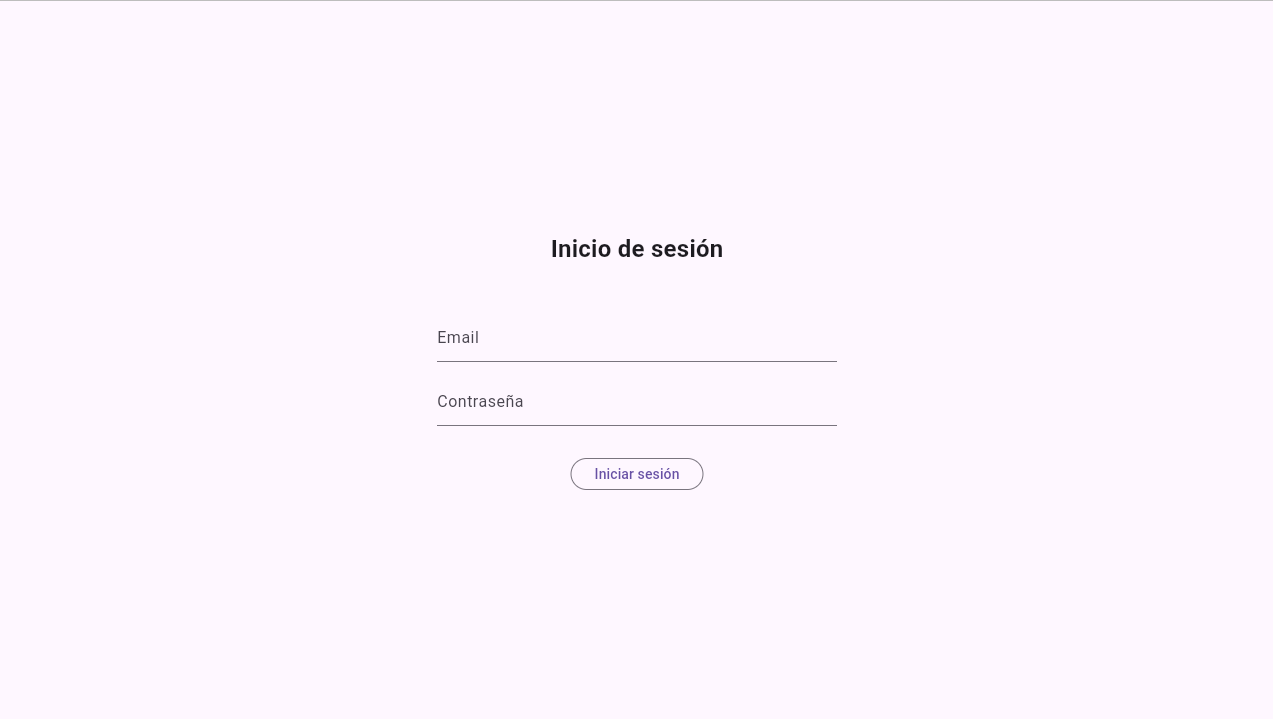
\includegraphics[width=0.7\textwidth]{imagenes/PrimeraIteracion/inicioSesion.png}
	\caption{Interfaz de usuario de inicio de sesión.}
	\label{fig:appInicioSesion}
\end{figure}

\subsubsection{Pantalla de principal}

\begin{figure}[H]
	\centering
	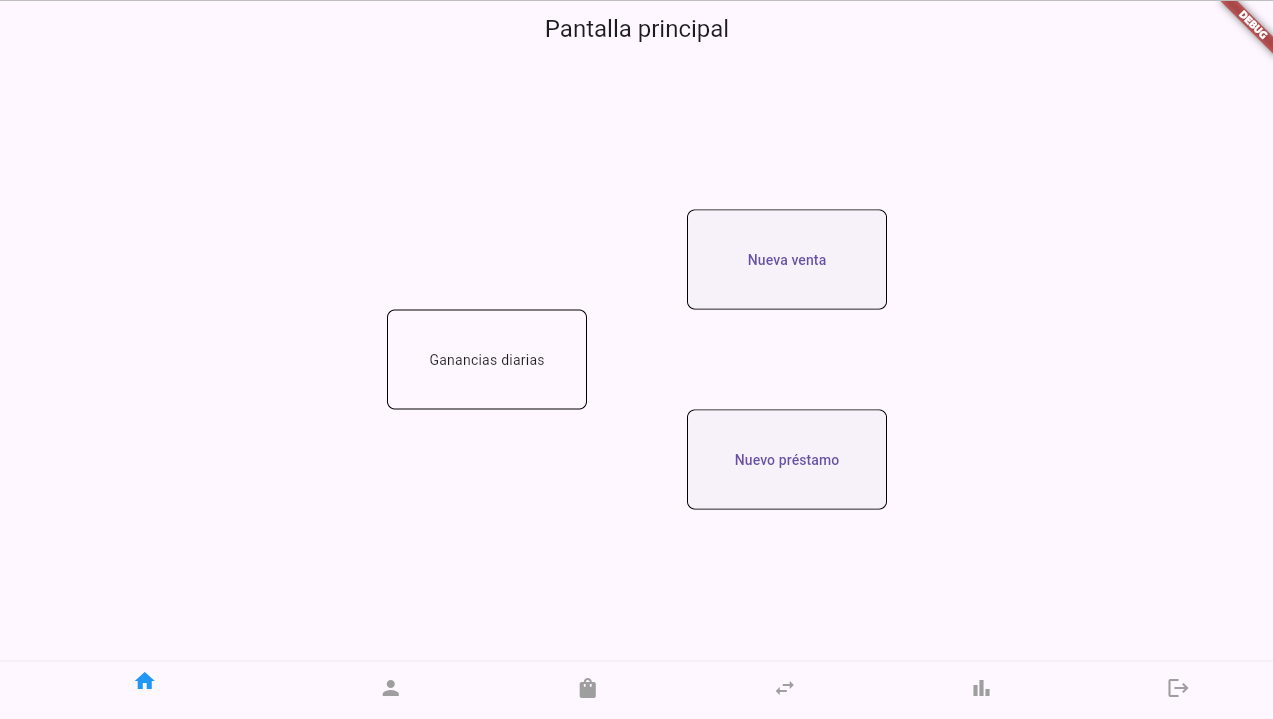
\includegraphics[width=0.7\textwidth]{imagenes/PrimeraIteracion/pantallaPrincipal.png}
	\caption{Interfaz de usuario de la pantalla principal.}
	\label{fig:appPantallaPrincipal}
\end{figure}

\subsubsection{Pantalla de visualización de clientes}

En esta pantalla se verán todos los clientes registrados en la tienda. Se pueden buscar por nombre o filtrar aquellos que deban dinero a la tienda. 

Los clientes que están en positivo en la tienda, es decir, tienen dinero a favor, se muestran con un fondo verde. Los clientes que están en negativo, se muestran con un fondo rojo. Si no tiene dinero a favor ni a deber, se muestran en blanco. 

\begin{figure}[H]
	\centering
	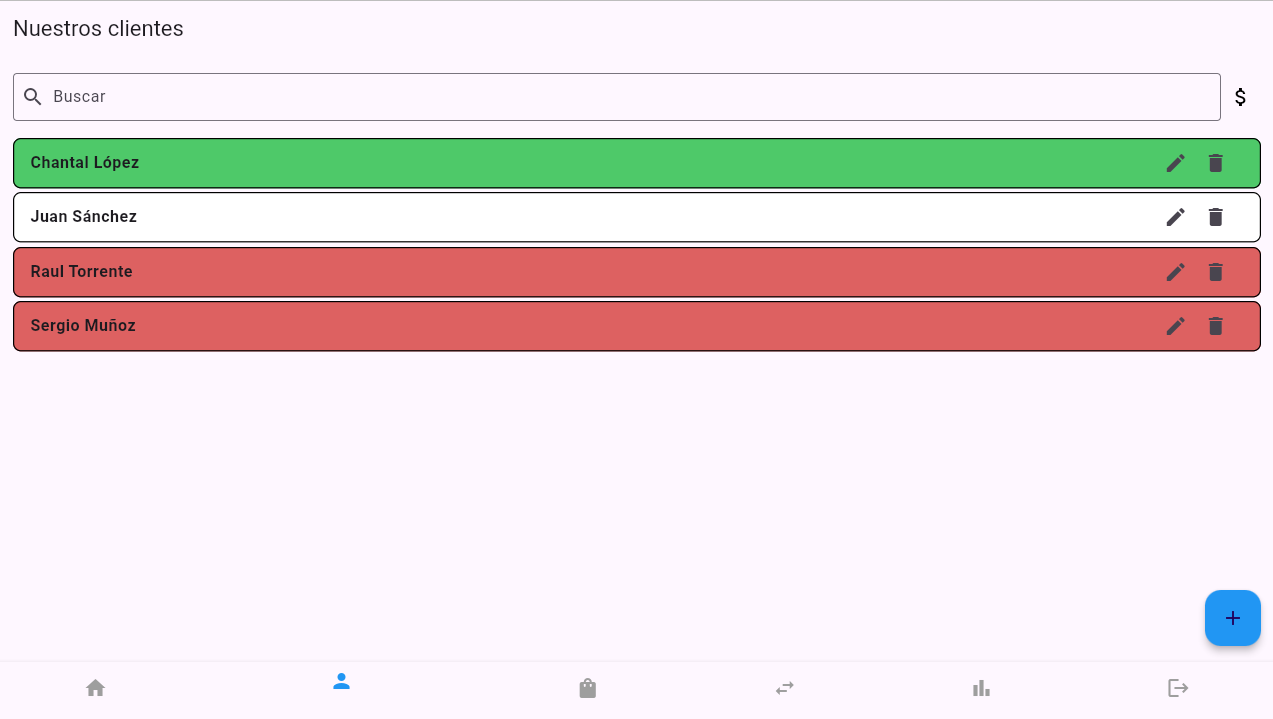
\includegraphics[width=0.7\textwidth]{imagenes/PrimeraIteracion/visualizacionClientes.png}
	\caption{Interfaz de usuario de la pantalla de visualización de clientes.}
	\label{fig:appVisualizarClientes}
\end{figure}

\subsubsection{Pantalla de añadir nuevo cliente}

\begin{figure}[H]
	\centering
	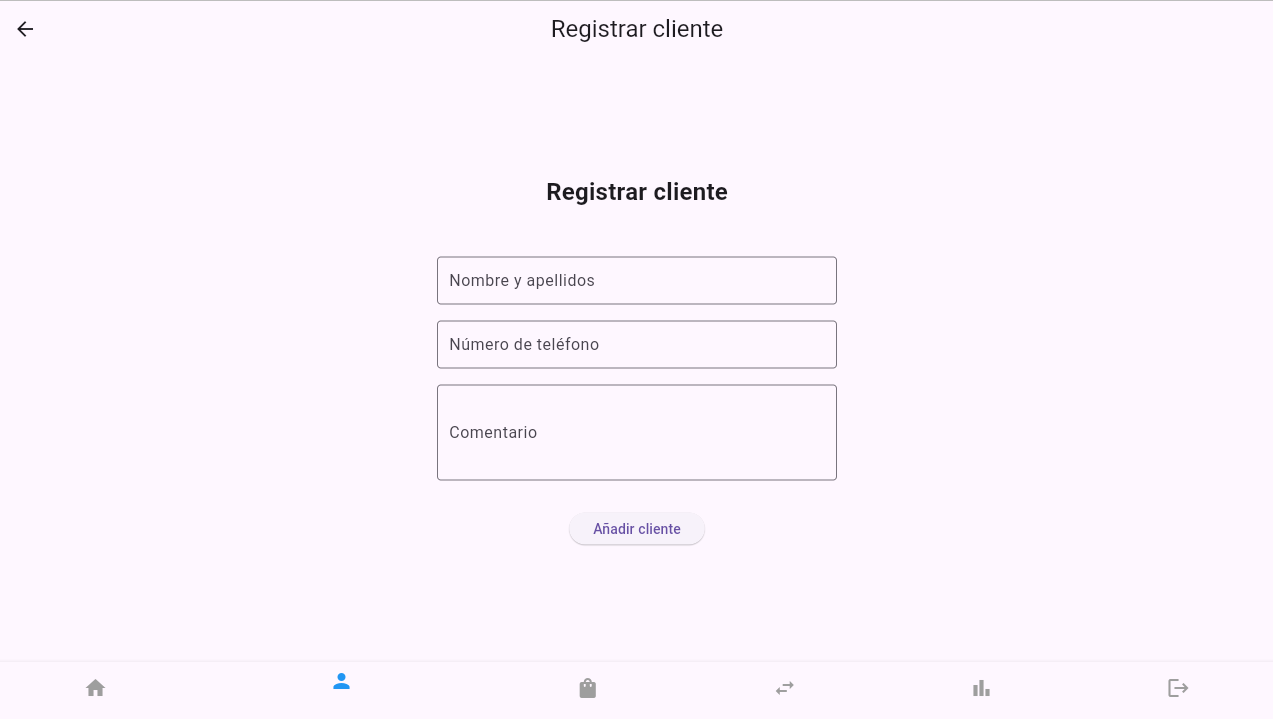
\includegraphics[width=0.7\textwidth]{imagenes/PrimeraIteracion/nuevoCliente.png}
	\caption{Interfaz de usuario de la pantalla de nuevo cliente.}
	\label{fig:appNuevoCliente}
\end{figure}

\subsubsection{Pantalla de editar un cliente existente}

\begin{figure}[H]
	\centering
	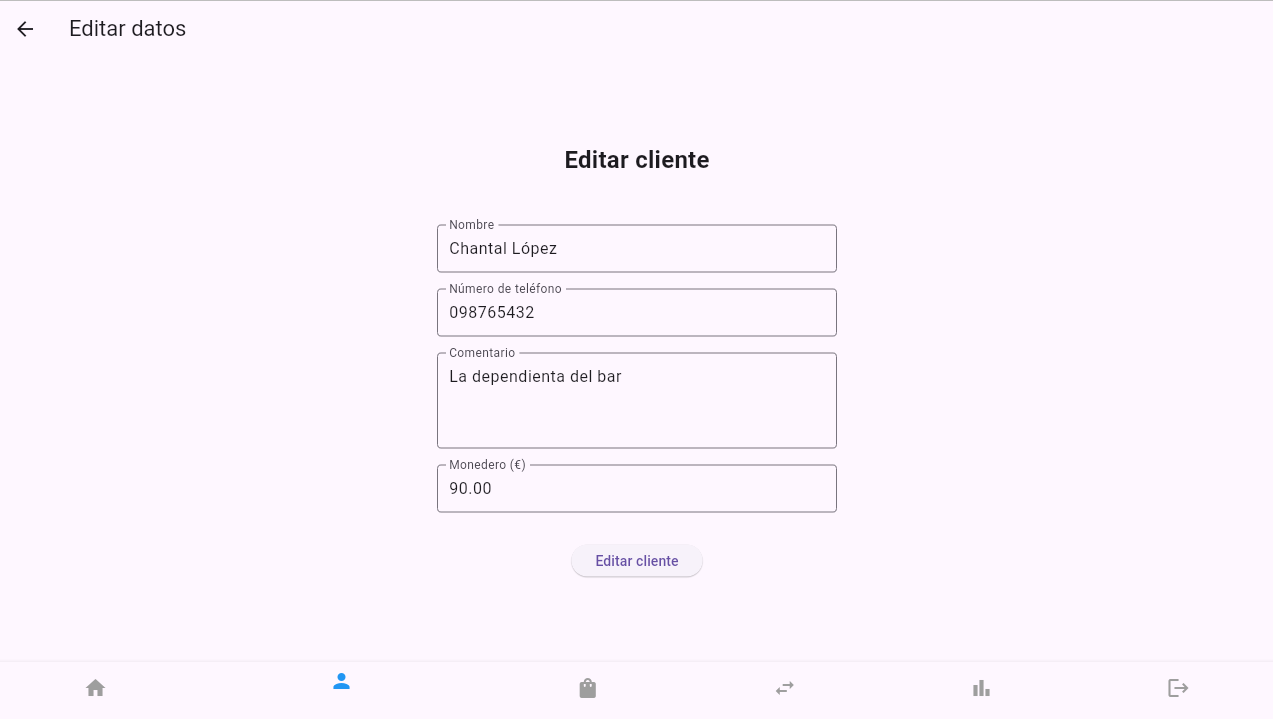
\includegraphics[width=0.7\textwidth]{imagenes/PrimeraIteracion/editarCliente.png}
	\caption{Interfaz de usuario de la pantalla de editar cliente.}
	\label{fig:appEditarCliente}
\end{figure}

\subsubsection{Pantalla de visualizar los datos de un cliente}

\begin{figure}[H]
	\centering
	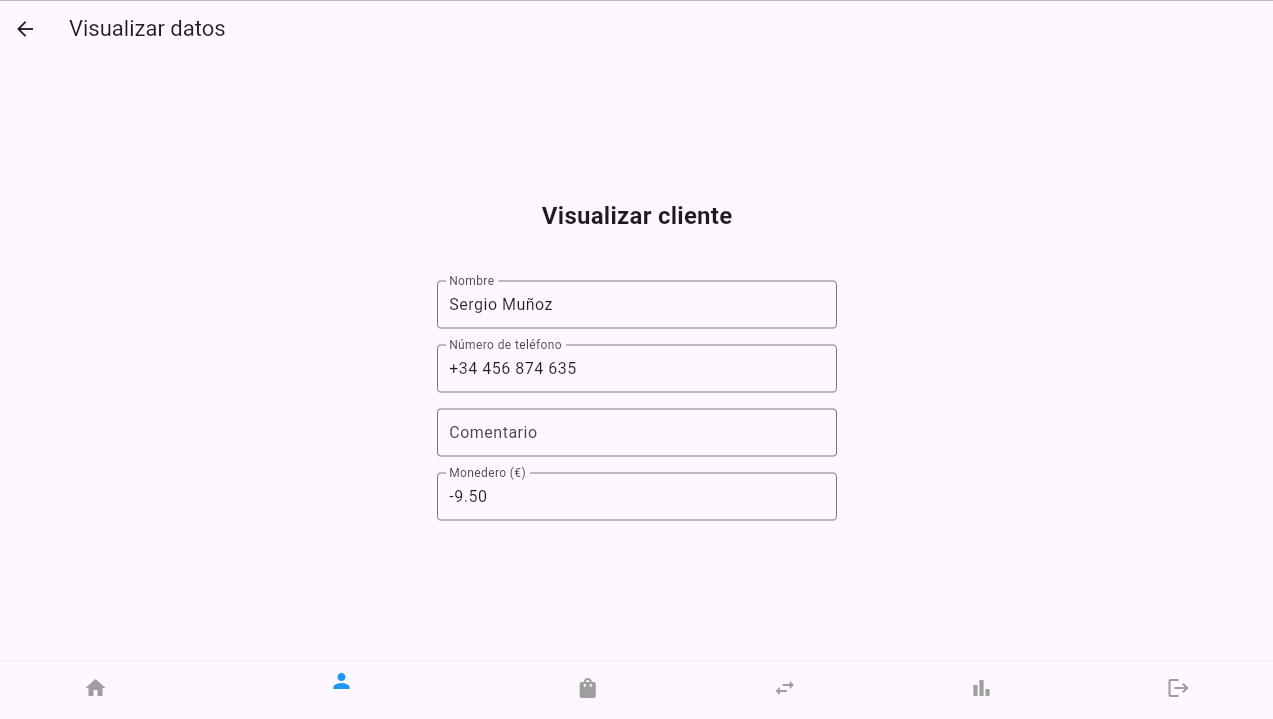
\includegraphics[width=0.7\textwidth]{imagenes/PrimeraIteracion/detallesCliente.png}
	\caption{Interfaz de usuario de la pantalla de visualizar datos de un cliente.}
	\label{fig:appDetallesCliente}
\end{figure}

\subsubsection{Pantalla de visualizar las categorías de artículos}

Se pueden añadir tantas categorías como el usuario crea conveniente para poder organizar los productos de su tienda a su gusto. 

\begin{figure}[H]
	\centering
	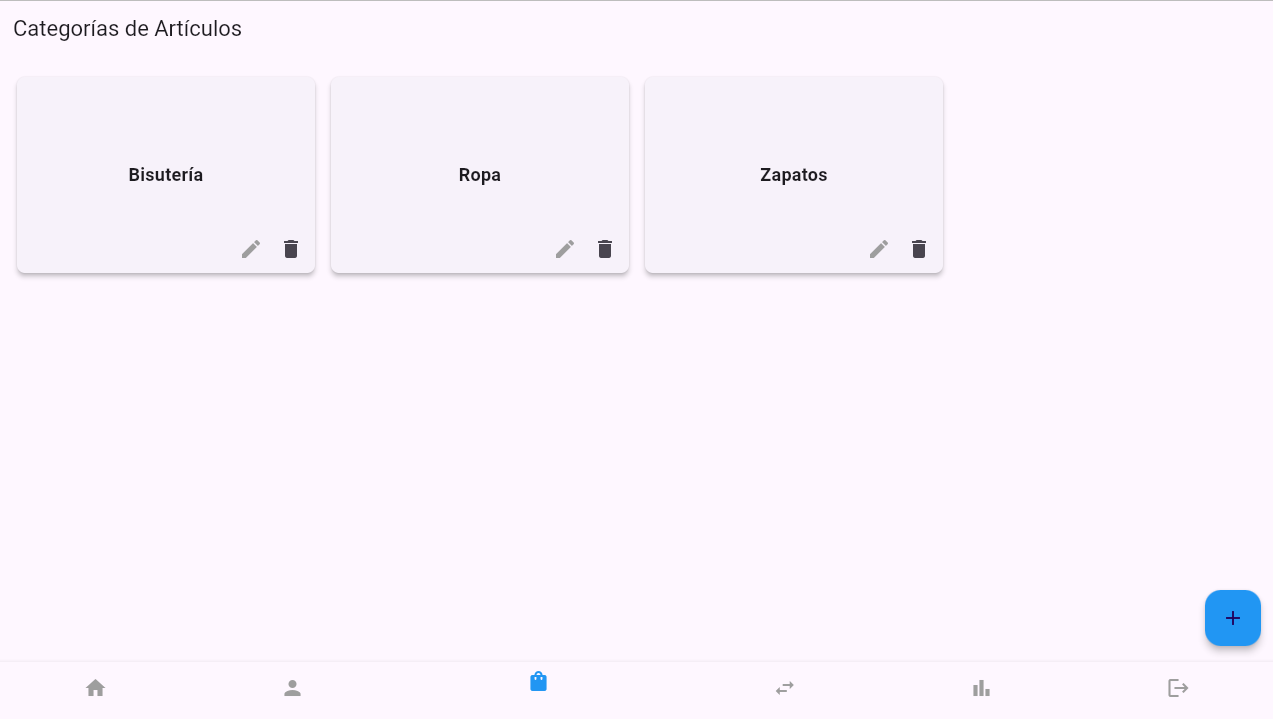
\includegraphics[width=0.7\textwidth]{imagenes/PrimeraIteracion/visualizarCategorias.png}
	\caption{Interfaz de usuario de la pantalla de visualizar las categorías.}
	\label{fig:appCategoriasArticulos}
\end{figure}

\subsubsection{Pantalla de añadir una nueva categoría de artículos}

Cuando se añade una nueva categoría, se deberá de especificar el nombre de dicha categoría y se podrán desmarcar los campos que no sean necesarios para esa categoría. Al marcar o desmarcar un campo, se cambia la visibilidad de este en todos los artículos que estén contenidos en esa categoría. Así se evita incluir campos que no tengan relevancia en ciertas categorías. 

\begin{figure}[H]
	\centering
	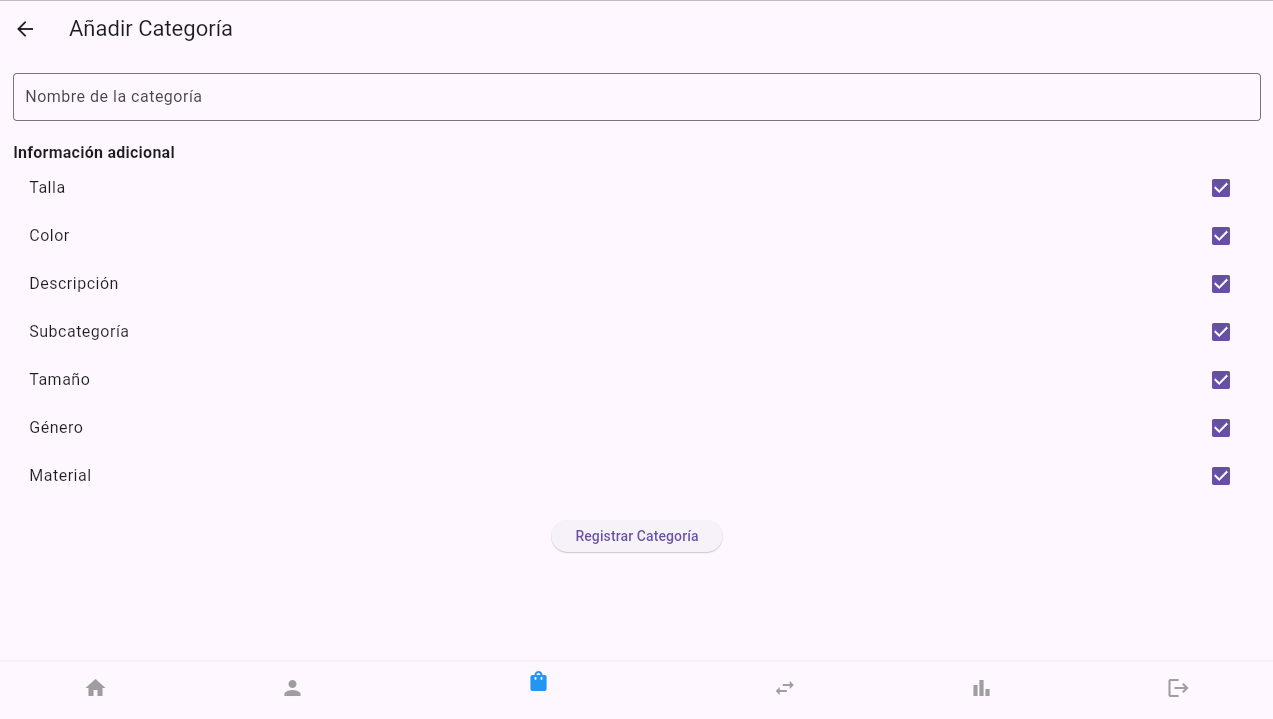
\includegraphics[width=0.7\textwidth]{imagenes/PrimeraIteracion/nuevaCategoria.png}
	\caption{Interfaz de usuario de la pantalla de añadir nueva categoría.}
	\label{fig:appNuevaCategoria}
\end{figure}

\subsubsection{Pantalla de editar una categoría existente}

\begin{figure}[H]
	\centering
	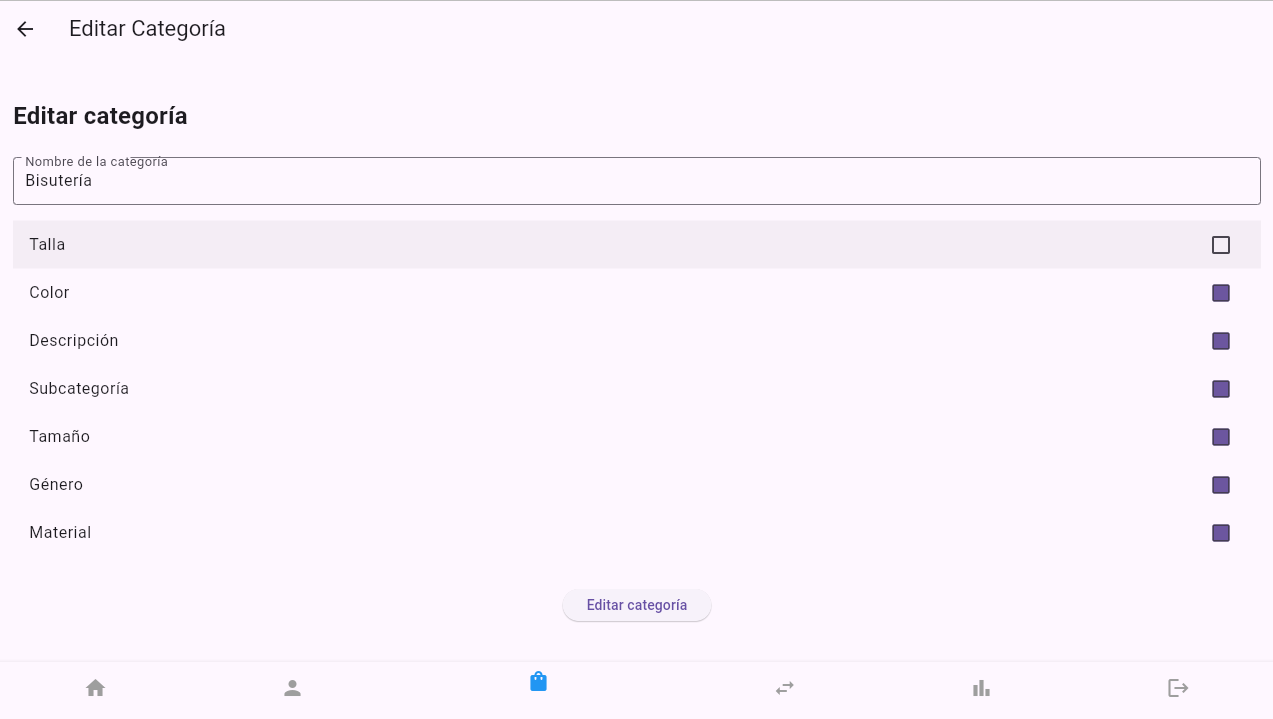
\includegraphics[width=0.7\textwidth]{imagenes/PrimeraIteracion/editarCategoria.png}
	\caption{Interfaz de usuario de la pantalla de editar una categoría.}
	\label{fig:appEditarCategoria}
\end{figure}

\subsubsection{Pantalla de visualizar los artículos de una categoría}

En esta pantalla se ven todos los artículos de una determinada categoría. Se puede buscar por nombre o filtrar por subcategoría. 

\begin{figure}[H]
	\centering
	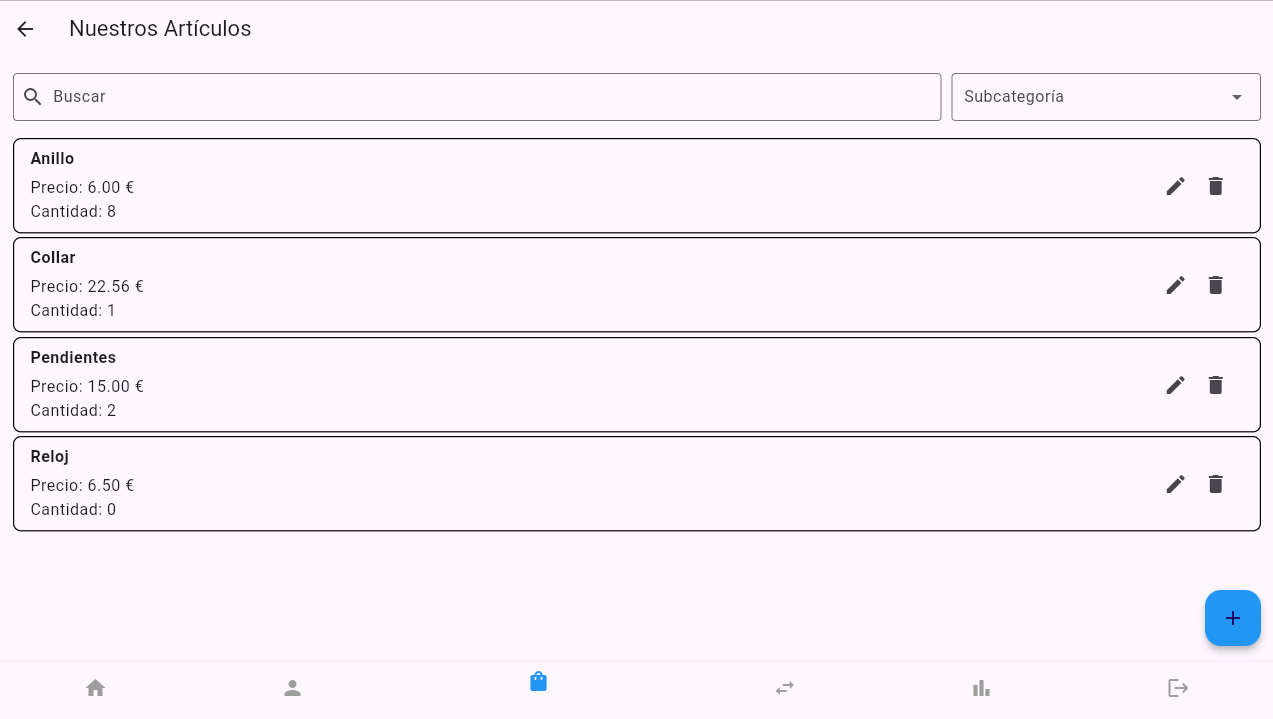
\includegraphics[width=0.7\textwidth]{imagenes/PrimeraIteracion/visualizarArticulos.png}
	\caption{Interfaz de usuario de la pantalla de visualizar artículos.}
	\label{fig:appVisualizarArticulos}
\end{figure}

\subsubsection{Pantalla de añadir un nuevo artículo a una categoría}

\begin{figure}[H]
	\centering
	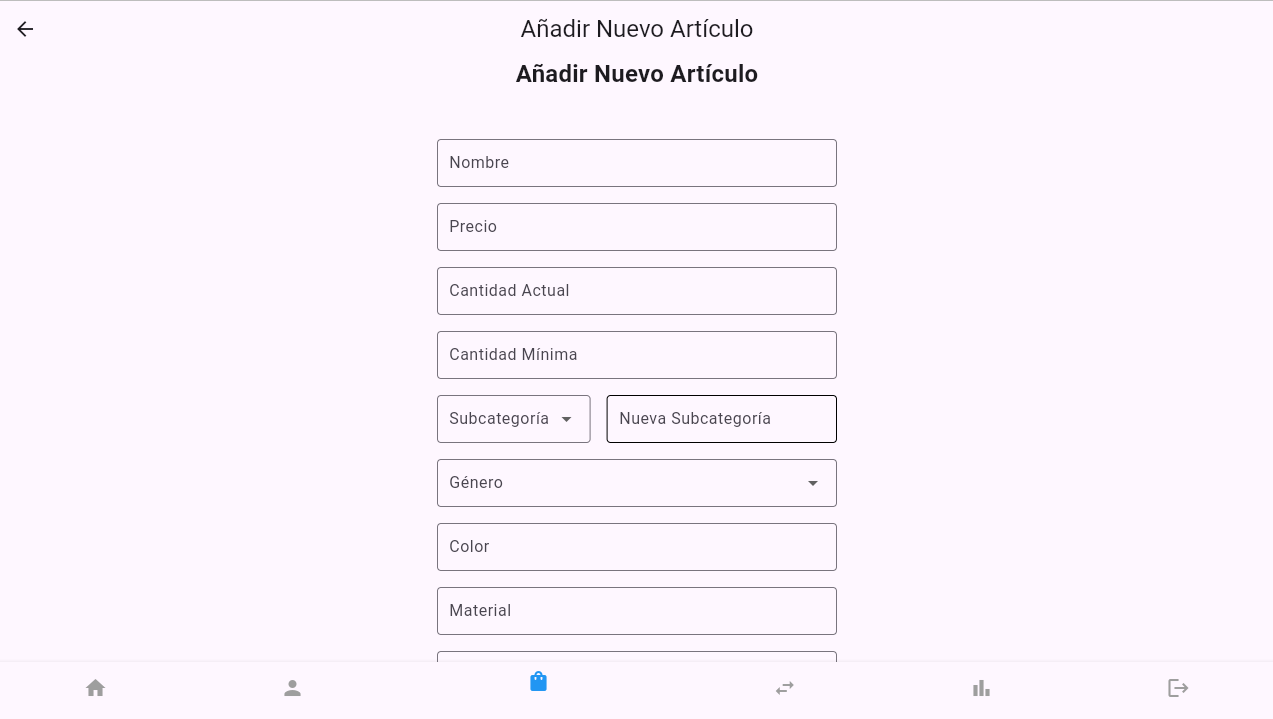
\includegraphics[width=0.7\textwidth]{imagenes/PrimeraIteracion/nuevoArticulo.png}
	\caption{Interfaz de usuario de la pantalla de añadir un nuevo artículo.}
	\label{fig:appNuevoArticulo}
\end{figure}

\subsubsection{Pantalla de editar un artículo existente de una categoría}

\begin{figure}[H]
	\centering
	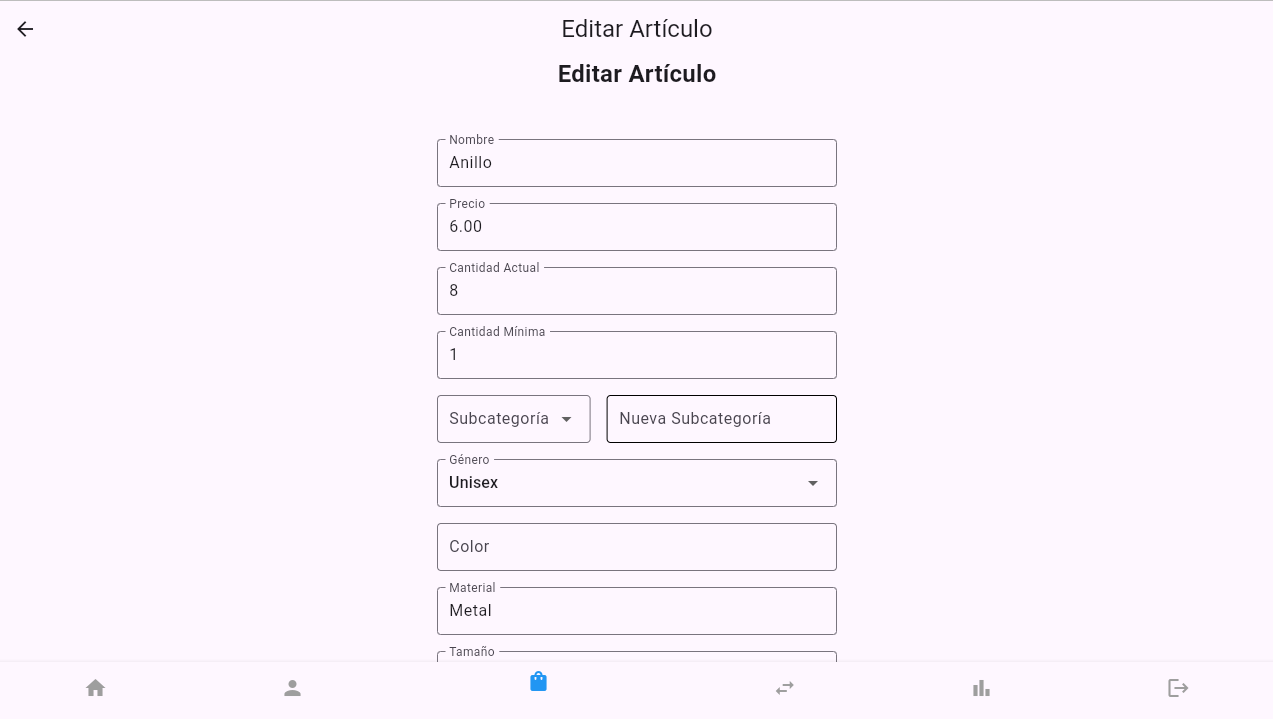
\includegraphics[width=0.7\textwidth]{imagenes/PrimeraIteracion/editarArticulo.png}
	\caption{Interfaz de usuario de la pantalla de editar un artículo existente.}
	\label{fig:appEditarArticulo}
\end{figure}

\subsection{Pruebas de funcionalidad}

Para testear la implementación que se ha llevado a cabo, se han realizado una serie de pruebas de funcionalidad: 

\begin{itemize}
	\item Comprobación de acceso a la aplicación únicamente con las credenciales válidas. 
	\item Comprobación de visualización de todos los clientes almacenados en la base de datos. 
	\item Comprobación del funcionamiento de búsqueda por nombre del cliente. 
	\item Comprobación del filtrado por deudas. 
	\item Comprobación de visualización de los detalles del cliente. 
	\item Comprobación de la edición de los datos del cliente. 
	\item Comprobación de la creación de un nuevo cliente. 
	\item Comprobación de la eliminación de un cliente existente. 
	\item Comprobación de la visualización de las categorías existentes en la tienda. 
	\item Comprobación de la creación de una nueva categoría en la tienda. 
	\item Comprobación de la edición de una categoría existente. 
	\item Comprobación de la visualización de los artículos vinculados con una categoría. 
	\item Comprobación de la búsqueda de un artículo por nombre. 
	\item Comprobación del filtrado de artículos según la subcategoría. 
	\item Comprobación de la visualización de las características un artículo. 
	\item Comprobación de la edición de las características de un artículo. 
	\item Comprobación del registro de un nuevo artículo. 
\end{itemize}




\subsection{Revisión de la iteración}

\subsubsection{Autenticación}

El cliente probó el sistema de autenticación y le pareció correcto. 

\subsubsection{Gestión de clientes}

El cliente probó este conjunto de pantallas que gestionan los clientes de la tienda. Pidió una mejora en la accesibilidad en la pantalla de visualizado de clientes. No diferenciar únicamente cuando un cliente debe con un sistema de colores (verde/rojo), añadir también un icono que lo represente. El resto de funcionalidades estaban correctas. 

\subsubsection{Gestión de artículos}

El cliente probó este conjunto de pantallas que gestionan los artículos de la tienda y decidió que no se estaban organizando de forma correcta. Las categorías estaban bien, pero a la hora de añadir nuevos artículos, el formulario debería de permitir añadir varias tallas, no únicamente una. Además, por cada talla, se debería de gestionar la cantidad actual, cantidad mínima y color. 

El resto de funcionalidades estaban bien.  


\subsection{Plan para la próxima iteración}

Para la próxima iteración se propone:

\begin{itemize}
	\item Implementar las mejoras señaladas por el cliente.
	\item Implementar la pantalla de la lista de renovación de artículos.
	\item Implementar las pantallas de gestión de movimientos.
\end{itemize}

\newpage

\section{Segunda iteración}

\subsection{Alcance de la iteración}

En esta segunda iteración se van a desarrollar los siguientes requisitos: RF10, RF19, RF20, RF21, RF22, RF23, RF24, RF25, RF26, RF27, RF28. 

Además se han mejorado los siguientes requisitos como consecuencia de las mejoras señaladas por el cliente: RF3, RF4, RF6.

\subsection{Implementación}

La implementación se ha llevado a cabo en relación a los diseños de los bocetos iniciales del capítulo anterior. Estos bocetos eran orientativos y el diseño se ha mejorado en esta etapa para obtener una mejor usabilidad. Tras completar la implementación, hemos obtenido las siguientes pantallas: 

\subsubsection{Pantalla principal}

En esta pantalla se pueden consultar las ganancias diarias y se muestran las opciones de generar una nueva venta o un nuevo préstamo. Esto se ha puesto en la pantalla principal ya que son las funcionalidades que se usarán con más frecuencia. 

\begin{figure}[H]
	\centering
	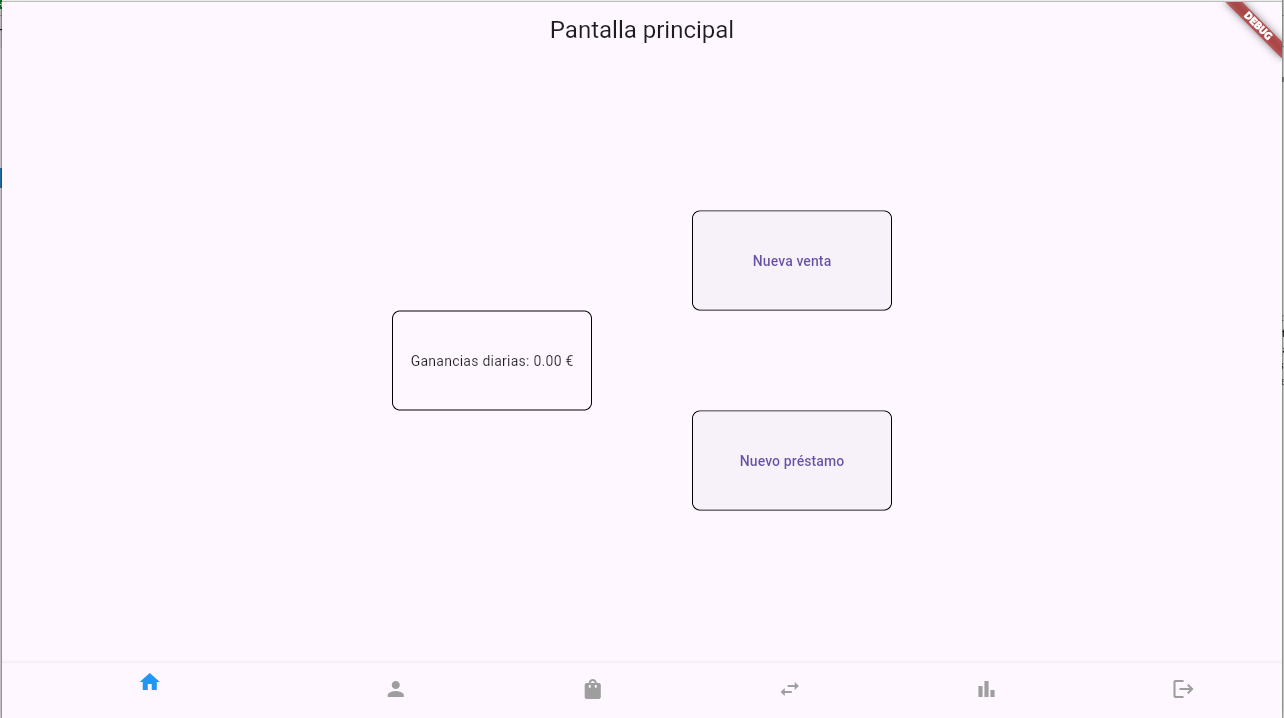
\includegraphics[width=0.7\textwidth]{imagenes/SegundaIteracion/pantallaPrincipal.png}
	\caption{Interfaz de usuario de la pantalla principal.}
	\label{fig:appPantallaPrincipal}
\end{figure}

\subsubsection{Pantalla de nueva venta}

En esta pantalla se realiza una nueva venta. En el buscador de la parte superior, se van proponiendo artículos que coincidan con los caracteres buscados. Una vez seleccionado el artículo, en los desplegables de la talla y el color, se proponen únicamente las tallas o colores que existan para dicho artículo. La cantidad no puede ser inferior a 1. Si la cantidad es mayor a la que hay disponible en la tienda, salta un error avisando de que la cantidad es errónea. Si todo es correcto, pulsando al + se añade el artículo a la lista. Como es una venta, asignar el cliente es opcional. También es una búsqueda dinámica como el buscador de los artículos. El método de pago es obligatorio y se podrá elegir entre Efectivo y Tarjeta. Una vez todos los campos estén completos y se pulse al botón de Aceptar, se generará un nuevo movimiento tipo Venta.

\begin{figure}[H]
	\centering
	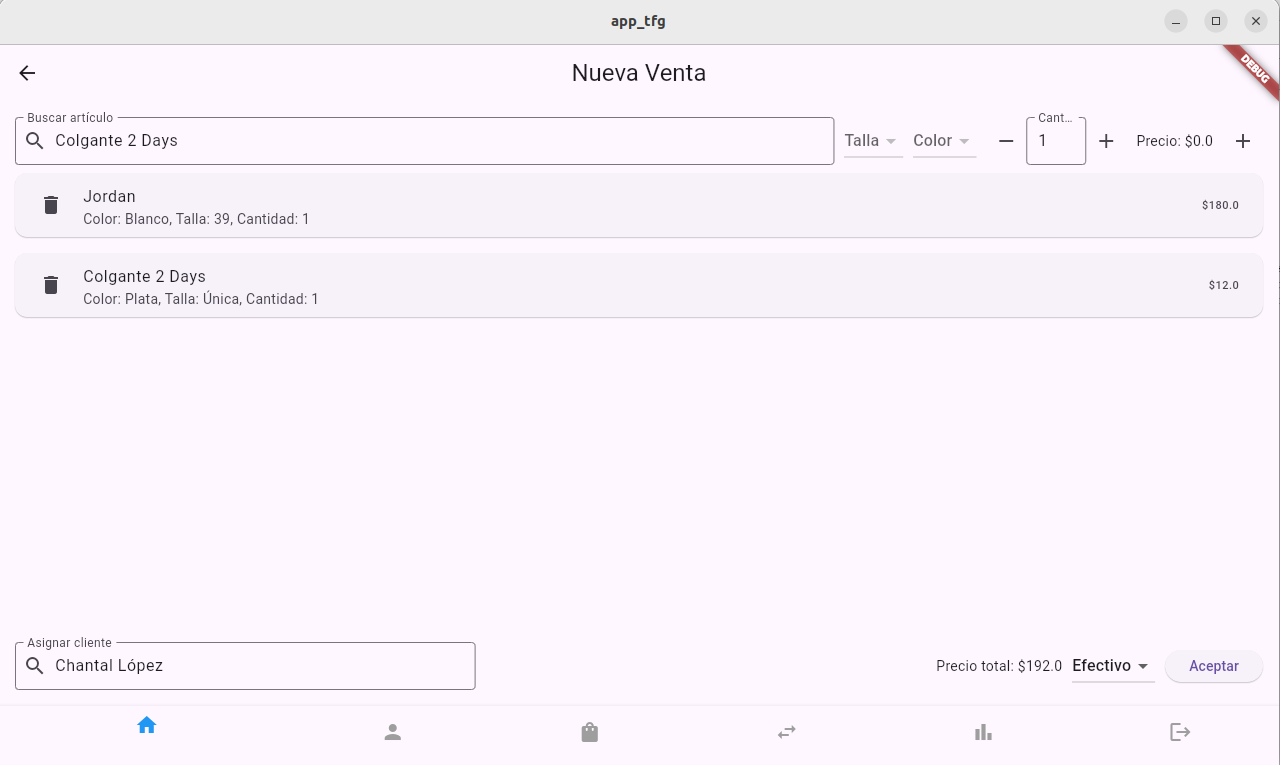
\includegraphics[width=0.7\textwidth]{imagenes/SegundaIteracion/nuevaVenta.png}
	\caption{Interfaz de usuario de la pantalla de nueva venta.}
	\label{fig:appPantallaNuevaVenta}
\end{figure}

\subsubsection{Pantalla de nuevo préstamo}

Esta pantalla funciona de la misma forma que la nueva venta. Sin embargo, asignar el cliente será obligatorio y el método de pago no existe ya que los préstamos no se pagan. El dinero de dicho préstamo se verá reflejado de forma negativa en el monedero del cliente. Además, se generará un movimiento de tipo Préstamo. 

\begin{figure}[H]
	\centering
	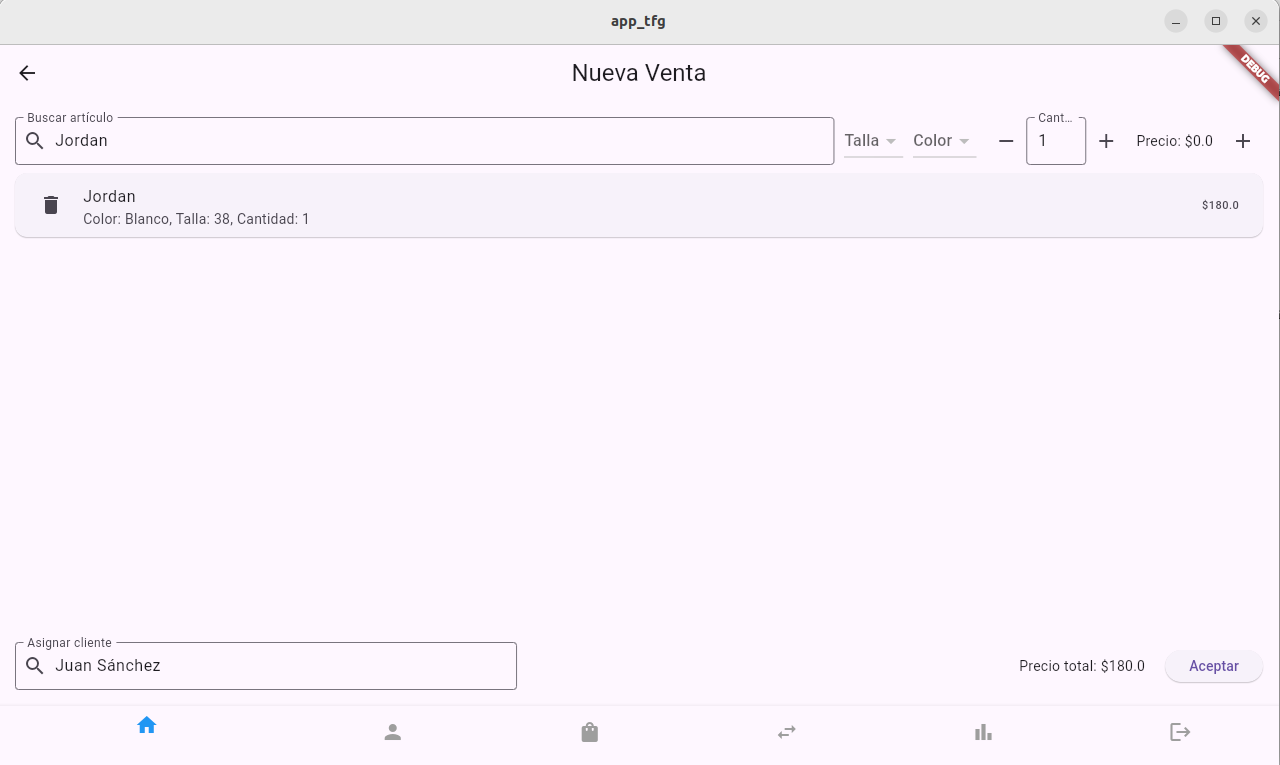
\includegraphics[width=0.7\textwidth]{imagenes/SegundaIteracion/nuevoPrestamo.png}
	\caption{Interfaz de usuario de la pantalla de nuevo préstamo.}
	\label{fig:appPantallaNuevoPrestamo}
\end{figure}

\subsubsection{Pantalla de visualización de movimientos}

En esta pantalla podemos ver todos los movimientos efectuados en la tienda. Están ordenados de forma que los más recientes se sitúen en la parte superior. Se puede eliminar un movimiento, pero se avisará de que el inventario no se actualizará. Esta funcionalidad es únicamente para permitir borrar movimientos que se generen por error. En la parte superior se puede buscar por cliente. Una vez seleccionado el cliente, solo aparecerán los movimientos que estén asociados a dicho cliente. Además, se puede filtrar por tipo de movimiento: Venta, Préstamo o Devolución. 

\begin{figure}[H]
	\centering
	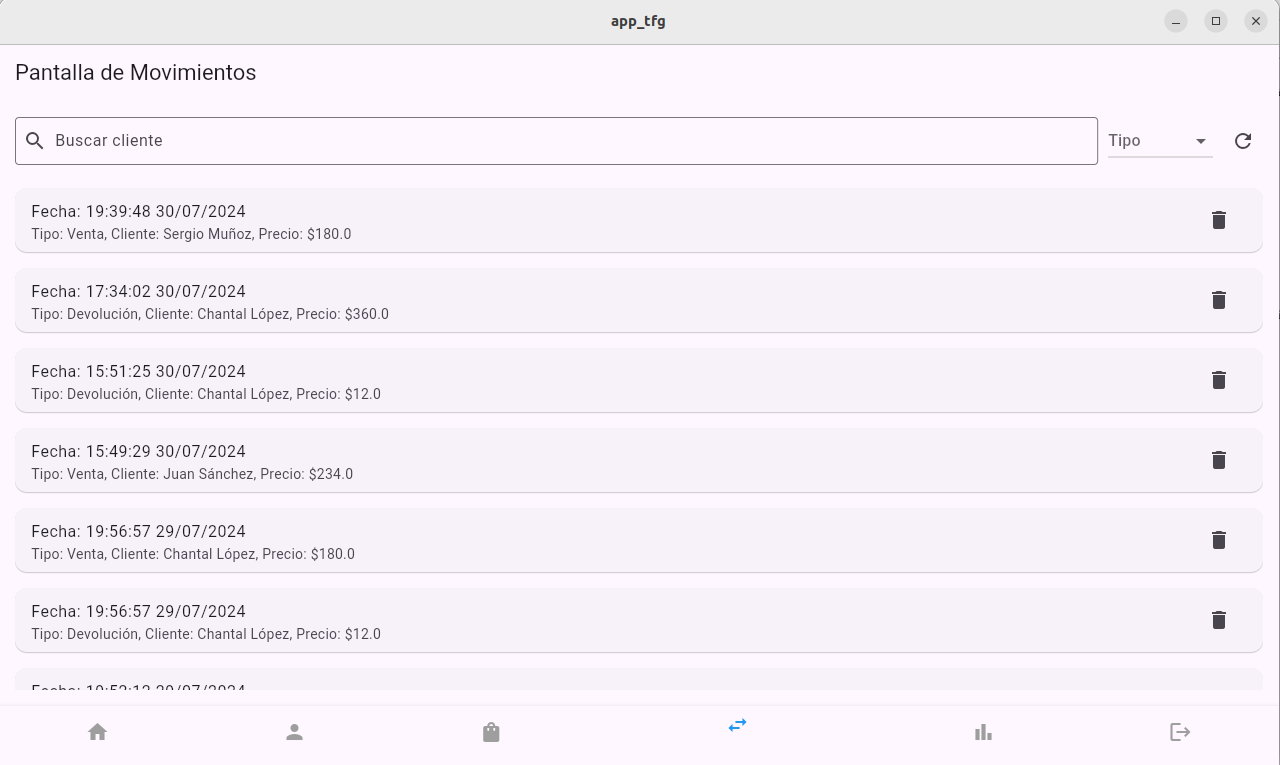
\includegraphics[width=0.7\textwidth]{imagenes/SegundaIteracion/listaMovimientos.png}
	\caption{Interfaz de usuario de la pantalla de visualización de movimientos.}
	\label{fig:appPantallaVisualizarMovimientos}
\end{figure}

\subsubsection{Pantalla de detalles del movimiento}

En esta pantalla podemos ver los detalles de un movimiento en específico. Esta pantalla muestra distintas funcionalidades dependiendo del tipo y del estado del movimiento. 

\textbf{Venta:} Cuando se trata de una venta, en la esquina superior derecha aparecen dos botones que te proponen una devolución parcial (solo quieres devolver algunos artículos) o una devolución total (se quieren devolver todos los artículos). Además, se pueden observar los datos relevantes de la venta, como los artículos involucrados, el cliente, el método de pago, la fecha y el precio total. 

\begin{figure}[H]
	\centering
	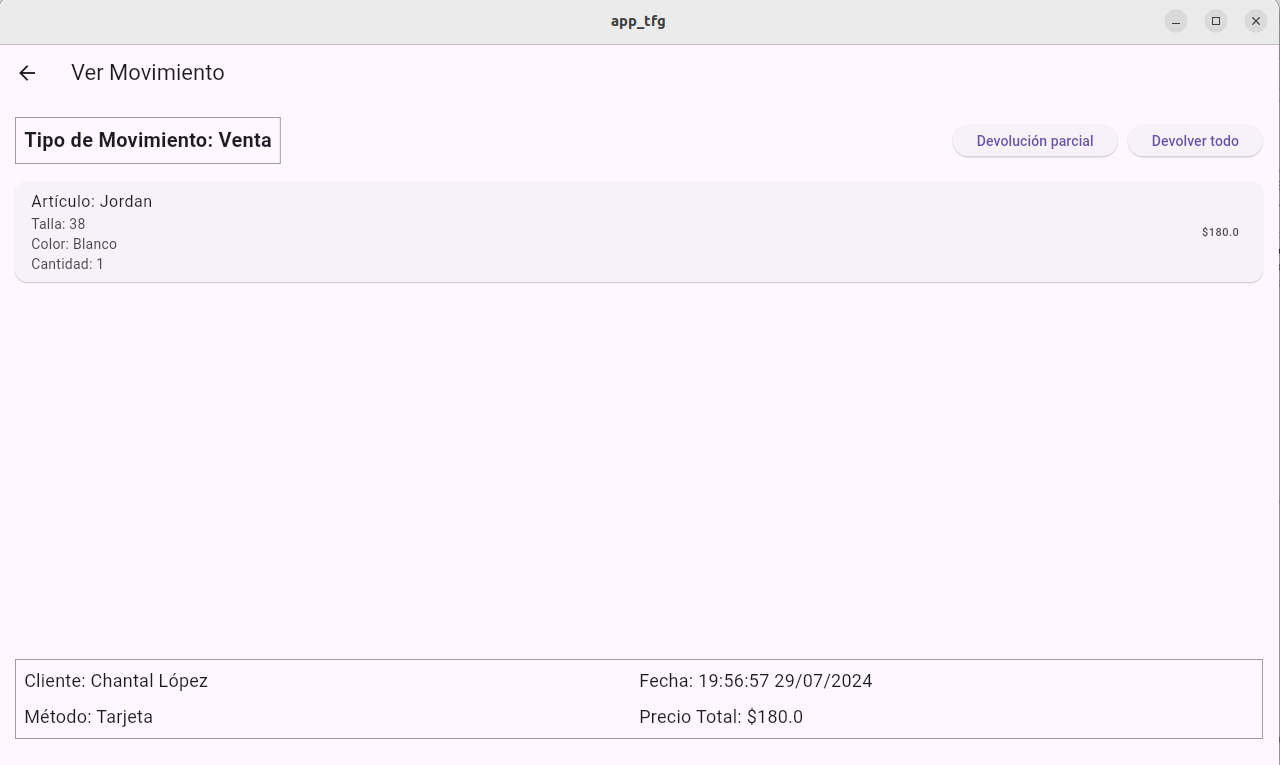
\includegraphics[width=0.7\textwidth]{imagenes/SegundaIteracion/detallesVenta.png}
	\caption{Interfaz de usuario de la pantalla de detalles de una venta.}
	\label{fig:appPantallaDetalleVenta}
\end{figure}

Si se realiza una devolución total, no se muestra ninguna pantalla adicional, directamente se crea un nuevo movimiento tipo Devolución con todos los artículos de la venta. Al realizar una devolución parcial, la pantalla cambia su modo Visualización a modo Devolución. Se permite escoger los artículos que se desean devolver y el método de pago en el que se prefiere realizar la devolución. 

\begin{figure}[H]
	\centering
	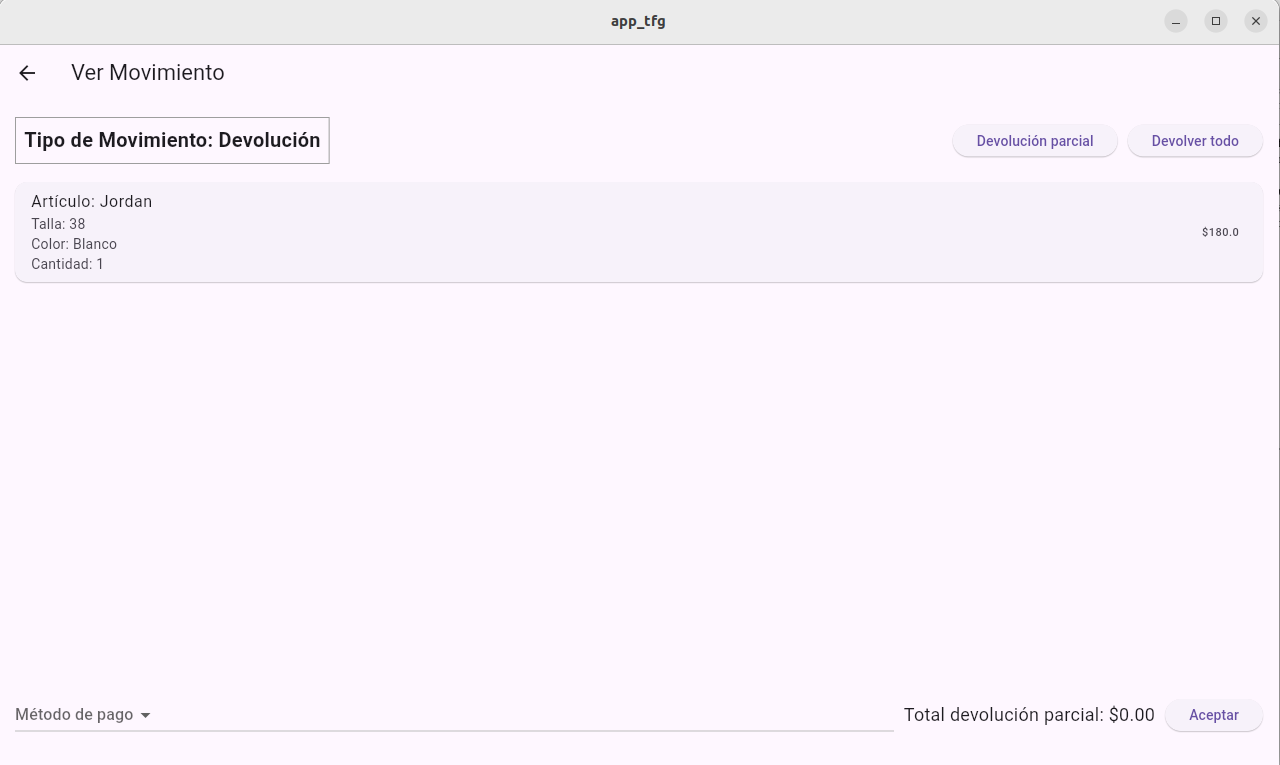
\includegraphics[width=0.7\textwidth]{imagenes/SegundaIteracion/devolucionVenta.png}
	\caption{Interfaz de usuario de la pantalla de devolución de una venta.}
	\label{fig:appPantallaDevolucionVenta}
\end{figure}

Tras aceptar la devolución, se genera un nuevo movimiento tipo Devolución. En la venta, se verá reflejada esta devolución. Desaparecen los botones de Devolución parcial y Devolución Total y aparece un botón con una referencia a la devolución realizada. De esta forma, se podrá visualizar de forma directa la devolución que se ha hecho de cada venta. 

\begin{figure}[H]
	\centering
	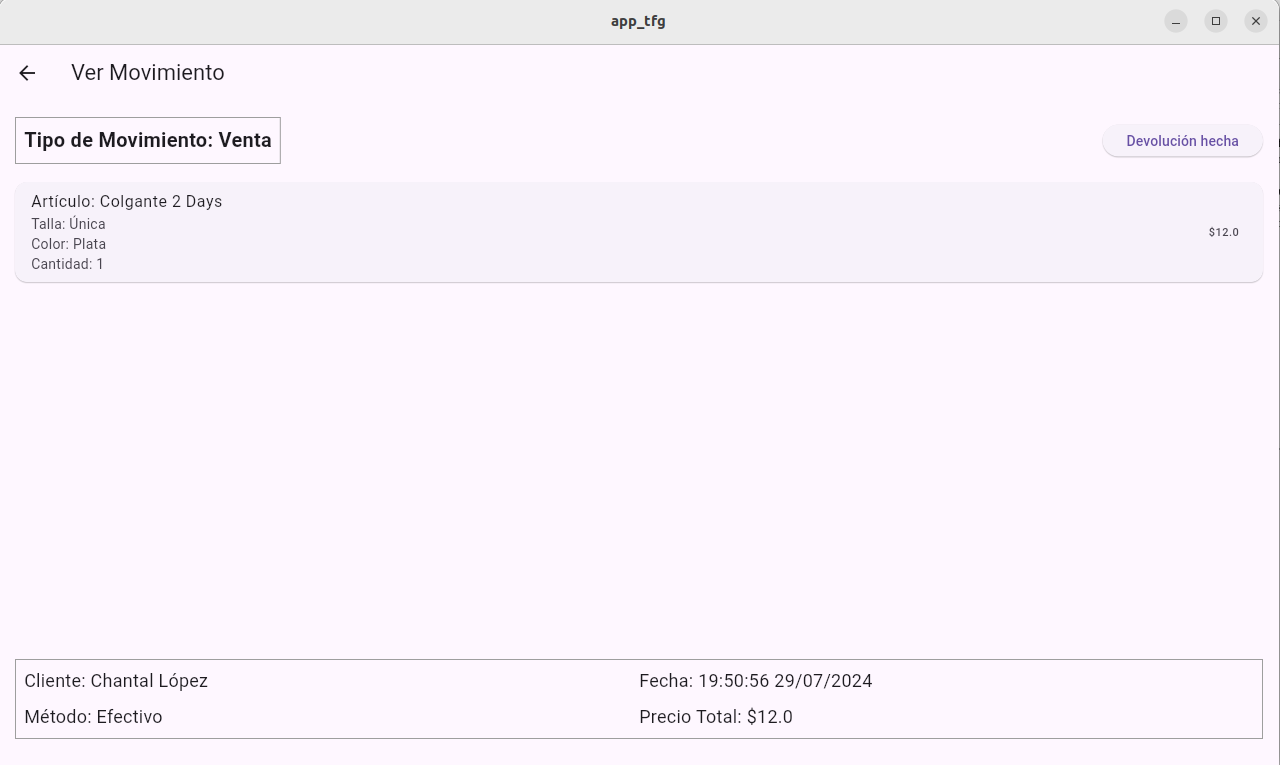
\includegraphics[width=0.7\textwidth]{imagenes/SegundaIteracion/devolucionHechaVenta.png}
	\caption{Interfaz de usuario de la pantalla de una venta con devolución hecha.}
	\label{fig:appPantallaDevolucionHechaVenta}
\end{figure}



\textbf{Pŕestamo: } La interfaz es similar a la pantalla de detalles de una venta, muestra la misma información. Sin embargo, los botones de la esquina superior son distintos. Una vez más, se ofrecen dos opciones: Compra o Devolver todo. El botón de Devolver todo funciona de la misma forma que en la Venta. 


\begin{figure}[H]
	\centering
	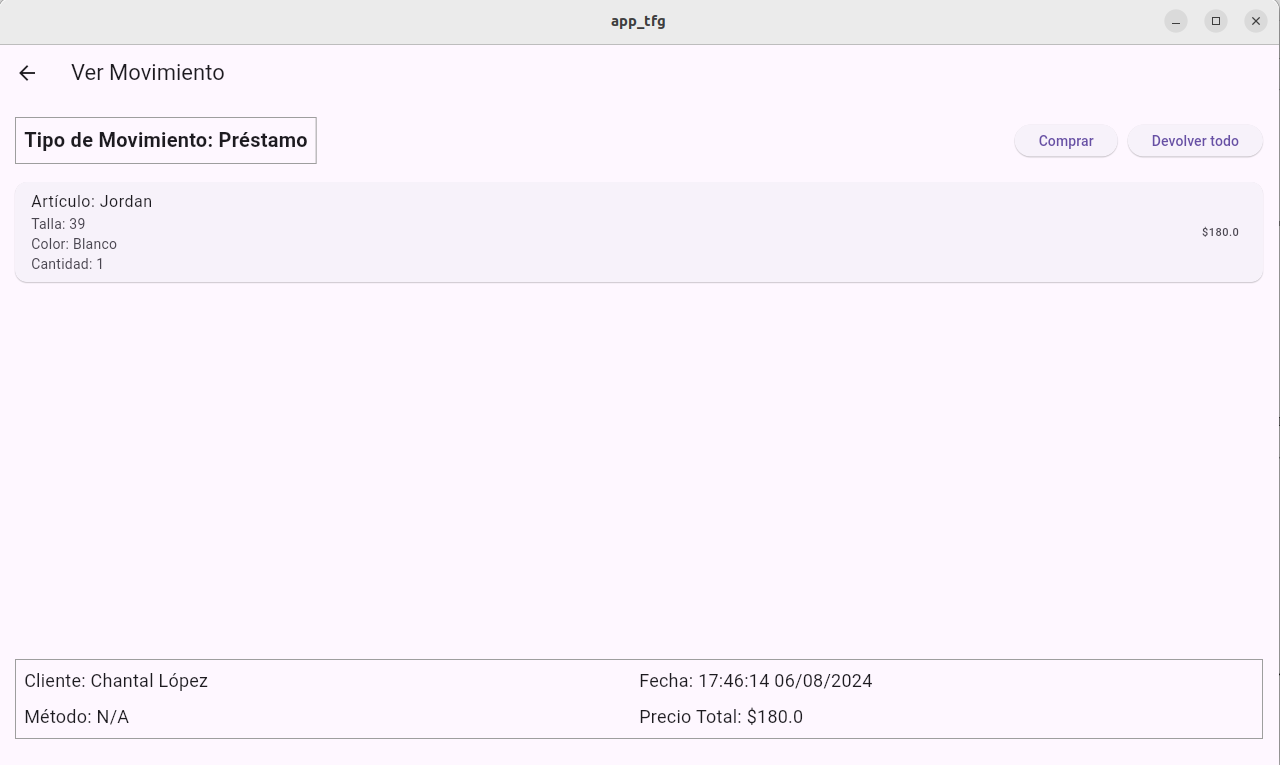
\includegraphics[width=0.7\textwidth]{imagenes/SegundaIteracion/detallesPrestamo.png}
	\caption{Interfaz de usuario de la pantalla los detalles de un préstamo.}
	\label{fig:appPantallaDetallesPrestamo}
\end{figure}

La funcionalidad del botón de Compra es distinta. Este botón permite generar una compra a partir de un préstamo. Al pulsar este botón, se cambia la funcionalidad de la pantalla y permite seleccionar los artículos que se desean comprar. Seleccionar el método de pago es obligatorio. Al seleccionar Aceptar, se generan dos movimientos: un movimiento de venta con los artículos que se han seleccionado para comprar y un movimiento de devolución con aquellos artículos que no se hayan comprado (en el caso de que queden artículos sin seleccionar). Así se verá reflejado en el historial de la tienda aquellos artículos que se compran y se devuelven. A su vez, el inventario se actualiza con estos movimientos. 

\begin{figure}[H]
	\centering
	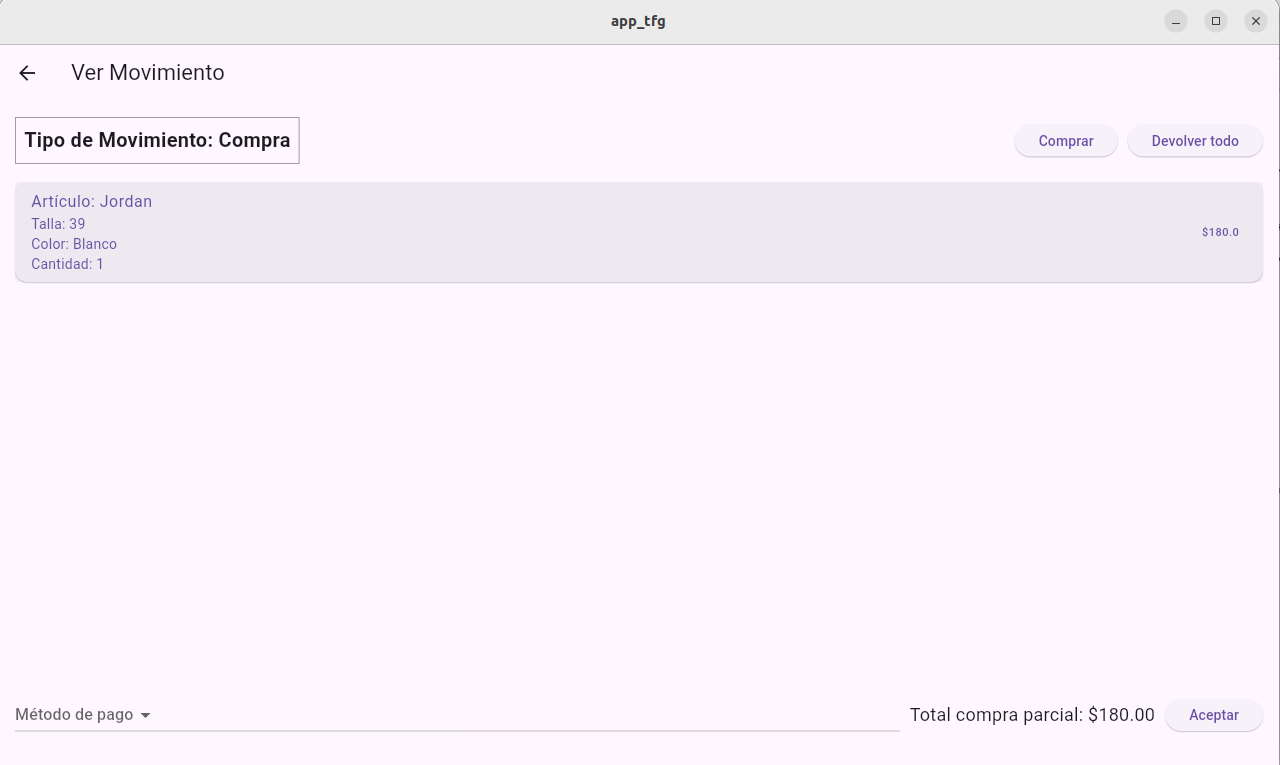
\includegraphics[width=0.7\textwidth]{imagenes/SegundaIteracion/compraPrestamo.png}
	\caption{Interfaz de usuario de la pantalla de compra a partir de un préstamo.}
	\label{fig:appPantallaCompraPrestamo}
\end{figure}

Si se ha hecho una devolución, se le asocia al préstamo de la misma forma que vimos en la venta.

\newpage

\textbf{Devolución: } Esta pantalla también muestra la misma información que los dos movimientos anteriores, los detalles del movimiento. En la esquina superior siempre aparecerá un botón de Movimiento original, que te llevará de forma directa al movimiento del cual proviene dicha devolución. 

\begin{figure}[H]
	\centering
	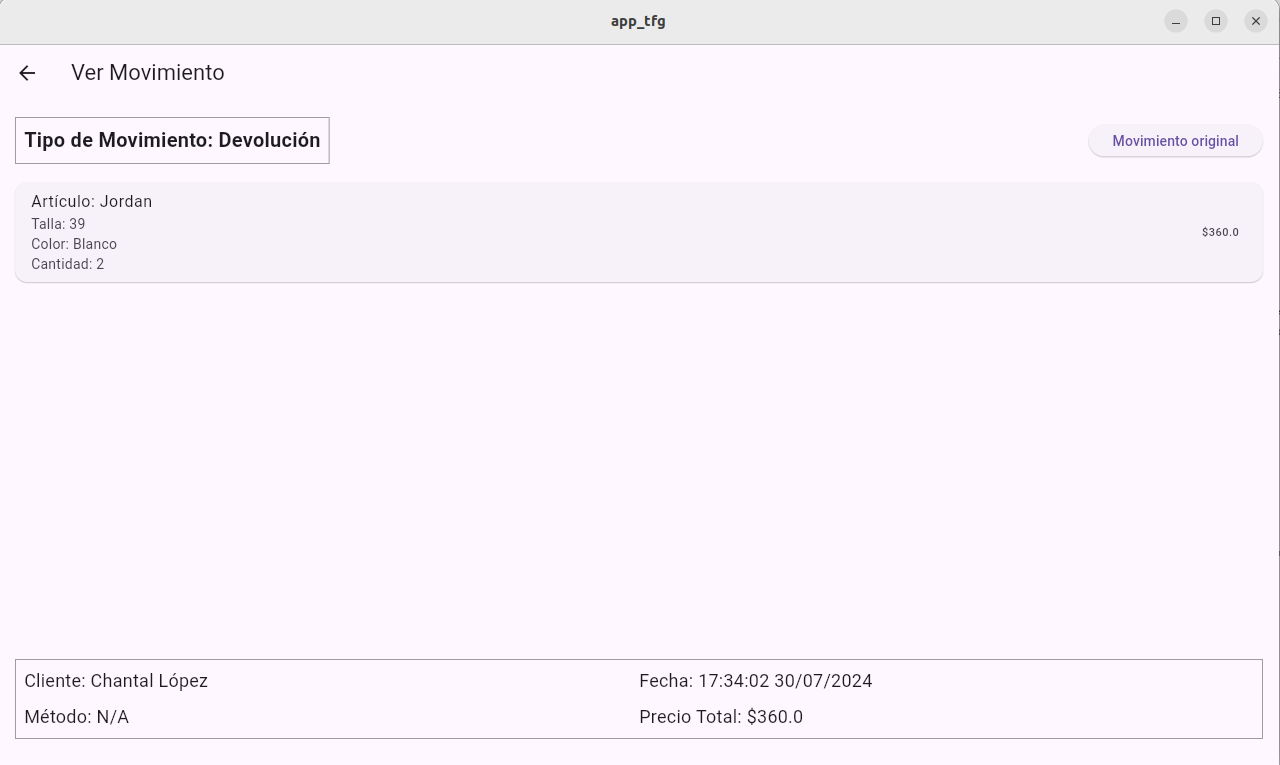
\includegraphics[width=0.7\textwidth]{imagenes/SegundaIteracion/detallesDevolucion.png}
	\caption{Interfaz de usuario de la pantalla de detalles de una devolución.}
	\label{fig:appPantallaDetallesDevolucion}
\end{figure}

\subsubsection{Mejora de las tallas en artículos}

En la iteración anterior, el cliente pidió que la gestión de las tallas de un artículo se hiciera de forma distinta. Se pidió que para cada artículo se pudieran añadir varias tallas. Para conseguir esto, se modifico la forma de crear un artículo, editarlo y visualizarlo. En la siguiente imagen podemos ver cómo la modificación ha sido correctamente efectuada. 

\begin{figure}[H]
	\centering
	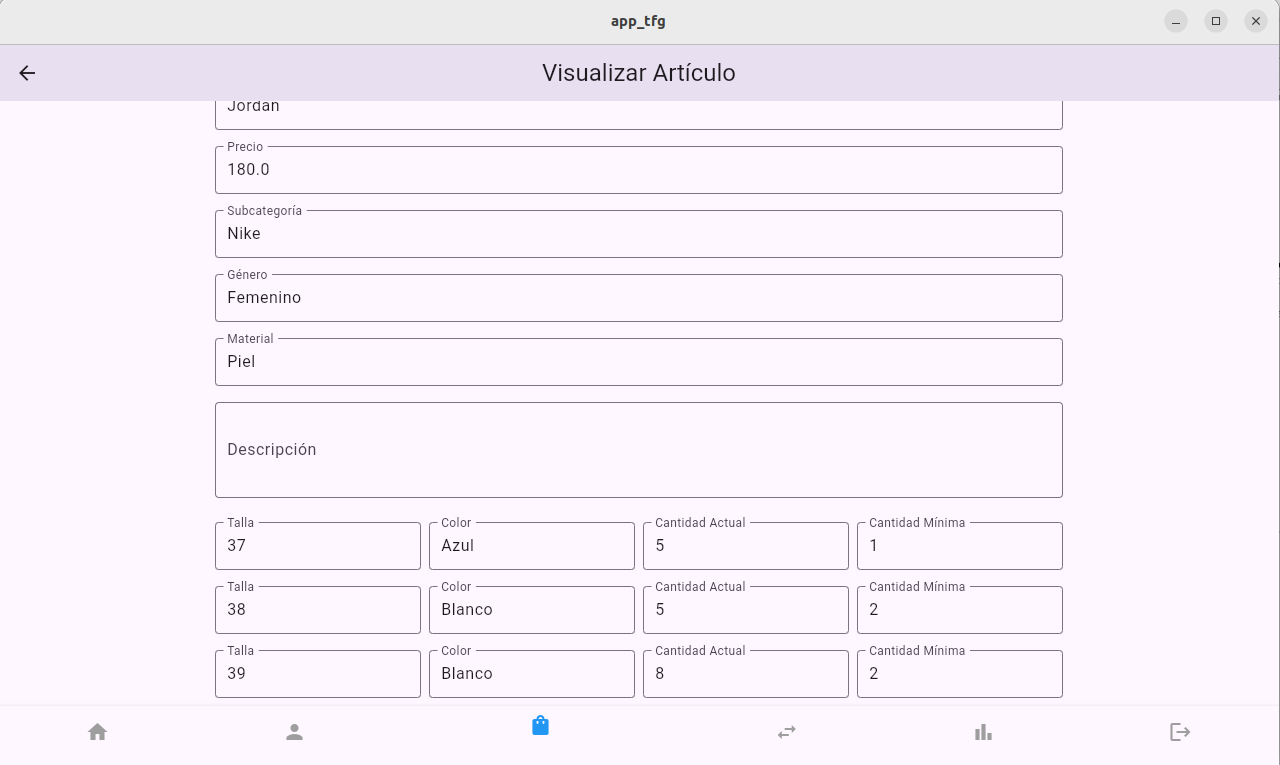
\includegraphics[width=0.7\textwidth]{imagenes/SegundaIteracion/tallasMultiples.png}
	\caption{Interfaz de usuario que muestra el cambio de la gestión de las tallas.}
	\label{fig:appPantallaDetallesDevolucion}
\end{figure}


\subsection{Pruebas de funcionalidad}

Para testear la implementación que se ha llevado a cabo, se han realizado una serie de pruebas de funcionalidad: 

\begin{itemize}
	\item Comprobación de la creación de una nueva venta. Esto implica que se almacenen los parámetros correctos y los artículos de dicha venta se almacenen en su tabla correspondiente. 
	\item Comprobación de la creación de un nuevo préstamo, prestando atención a que se cumplan sus características. 
	\item Comprobación de la visualización de todos los movimientos almacenados en al base de datos. 
	\item Comprobación de la eliminación de un movimiento. 
	\item Comprobación de la búsqueda de un movimiento por cliente. 
	\item Comprobación del filtrado de movimientos según su tipo. 
	\item Comprobación de visualización de los detalles de un movimiento. 
	\item Comprobación de la devolución total de una venta o préstamo. 
	\item Comprobación de la modificación de la cartera de un cliente tras la creación, eliminación o devolución de un préstamo. 
	\item Comprobación de la devolución parcial de una venta. 
	\item Comprobación de la realización de una compra a partir de un préstamo. 
	\item Comprobación de la navegación entre dos movimientos relacionados. 
	\item Comprobación de la correcta implementación de las tallas de un artículo. 
\end{itemize}


\subsection{Revisión de la iteración}

El cliente probó el sistema ideado para los movimientos y expresó que estaba conforme con la lógica de la implementación. Además, mostró gratitud por el cambio de las tallas que solicitó en la iteración anterior. 

Por tanto, el cliente no puso ninguna objeción y animó a continuar con el planning establecido. 

\subsection{Plan para la próxima iteración}

Para la próxima iteración se propone: 

\begin{itemize}
	\item Implementar la pantalla de gráficos.
	\item Mejorar la interfaz gráfica, realizando a su vez, mejoras en la usabilidad y accesibilidad.
	\item Testeo de posibles fallos de funcionamiento de la aplicación.
\end{itemize}

\section{Tercera iteración}

\subsection{Alcance de la iteración}

En esta iteración se llevarán a cabo los siguientes requisitos: RF29, RNF3 y RNF4. 

El primero de ellos corresponde con la creación de la pantalla de gráficos. Los últimos son requisitos no funcionales de usabilidad y accesibilidad. Debido a que en esta iteración se mejorará la interfaz gráfica de usuario, se tendrá en cuenta la mejora de la usabilidad y la accesibilidad. 

\subsection{Pantalla de gráficos}

Esta es la última pantalla que quedaba por implementar para completar el funcionamiento total de la aplicación. Como podemos observar, en la esquina superior de la pantalla hay un desplegable que permite adaptar la gráfica generada en función de si queremos que sea una gráfica mensual o anual. 

La gráfica mensual hace un resumen de las ganancias o pérdidas del mes actual. Además, se adapta al número de días que tenga el mes. 


\begin{figure}[H]
	\centering
	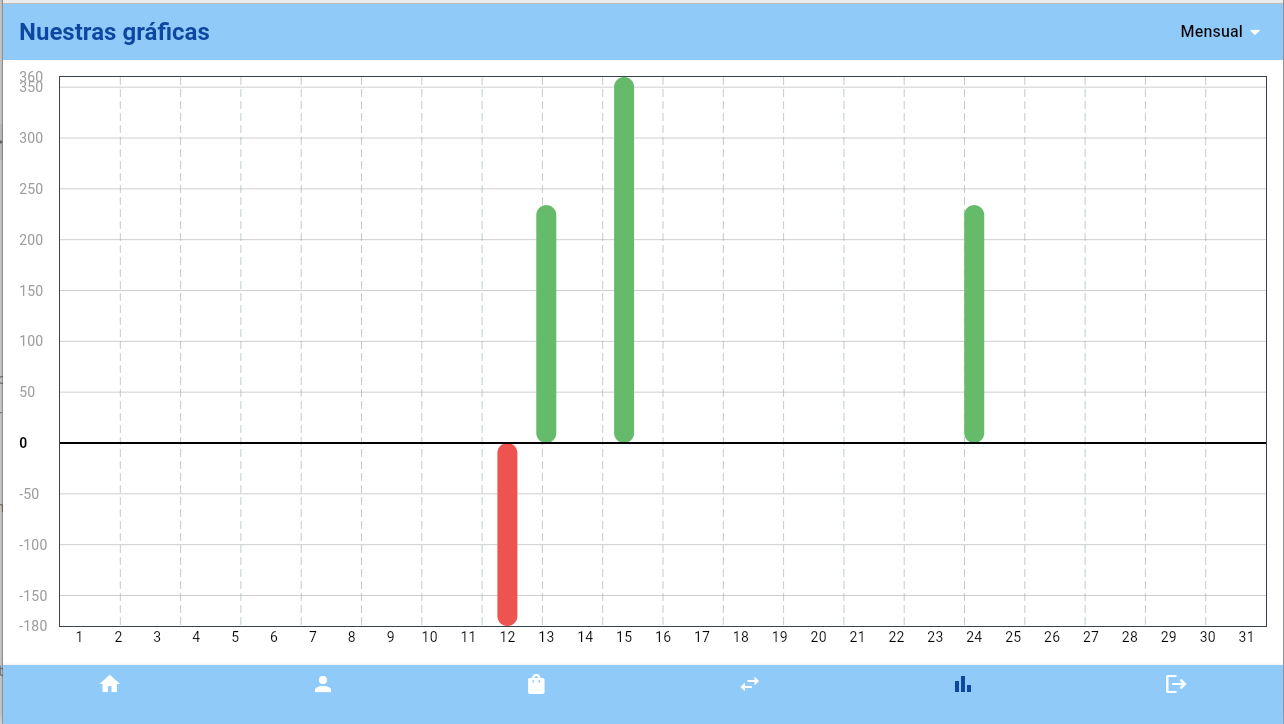
\includegraphics[width=0.7\textwidth]{imagenes/TerceraIteracion/graficosMensual.png}
	\caption{Pantalla de gráficos en modo Mensual.}
	\label{fig:mensual}
\end{figure}

La gráfica anual hace un resumen de las ganancias o pérdidas de año actual. Estas dos gráficas permiten obtener una visión general de progreso del negocio. 

\begin{figure}[H]
	\centering
	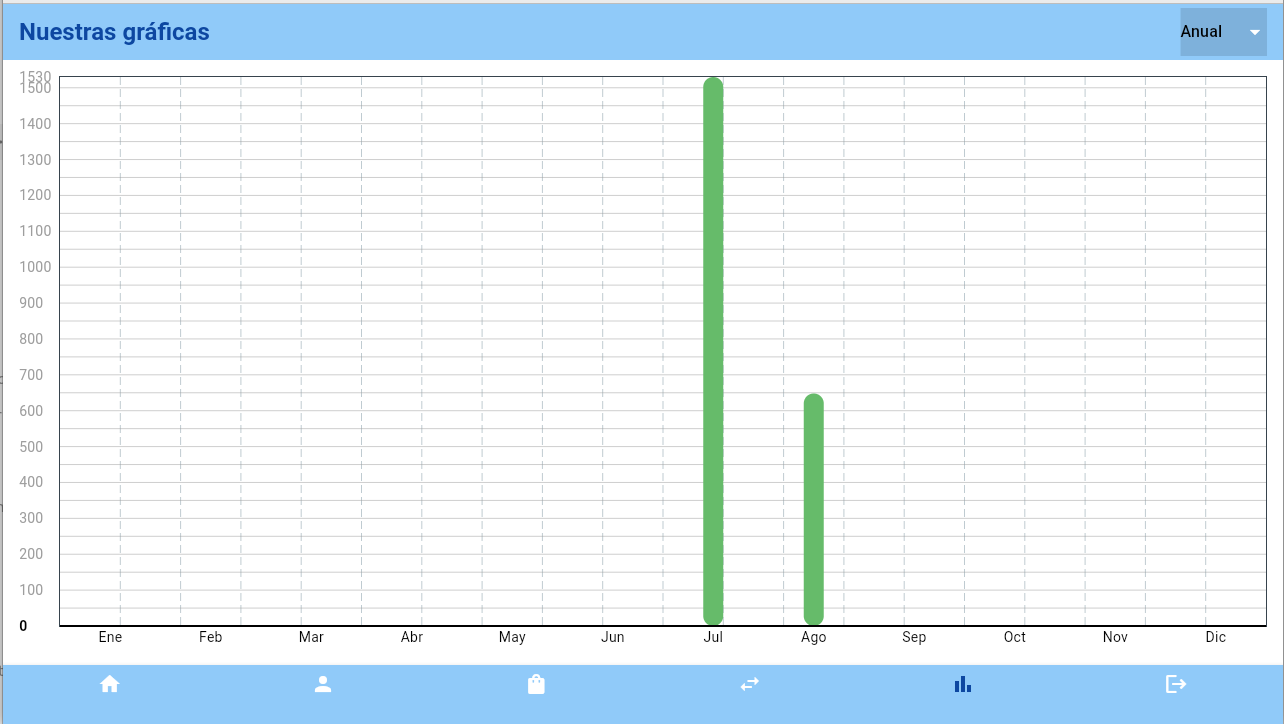
\includegraphics[width=0.7\textwidth]{imagenes/TerceraIteracion/graficosAnual.png}
	\caption{Pantalla de gráficos en modo Anual.}
	\label{fig:anual}
\end{figure}

Para hacer las cuentas y representarlas en las gráficas, únicamente se tienen en cuenta las ventas y las devoluciones. Los préstamos no se tienen en cuenta ya que es dinero que no ha sido recibido aún. 



\subsection{Mejora de la interfaz gráfica y la accesibilidad}

A lo largo de toda la aplicación, se mantiene: 

\begin{itemize}
	\item Un diseño sencillo e intuitivo para que sea usable.
	\item Fondos lisos y claros para facilitar la lectura del texto. 
	\item Fuente de letra estándar y colores que contrasten con el fondo.  
	\item Etiquetado de las pantallas para que el usuario pueda saber dónde está situado en cada momento. 
\end{itemize}

\subsection{Colores de la aplicación}

Para la interfaz de la aplicación se ha escogido como color primario el azul y como color secundario el amarillo. Estos dos colores son complementarios y hace que sea fácil llamar la atención del usuario realizando una buena combinación de ambos. 

Dentro del color primario, se ha trabajado con una gama de azules: 
\begin{itemize}
	\item \textbf{Azul claro:} Se ha seleccionado Colors.blue[50]. 
	\item \textbf{Azul medio:} Se ha seleccionado Colors.blue[200]. 
	\item \textbf{Azul oscuro:} Se ha seleccionado Colors.blue[900]. 
\end{itemize}

\begin{figure}[H]
	\centering
	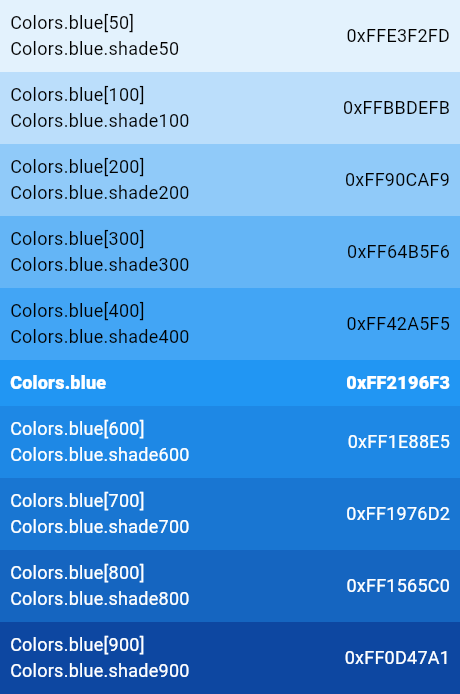
\includegraphics[width=0.33\textwidth]{imagenes/TerceraIteracion/ColorsBlue.png}
	\caption{Gama de colores azules de Flutter.}
\end{figure}


Como color secundario, se ha seleccionado Colors.yellow[600]. 

\begin{figure}[H]
	\centering
	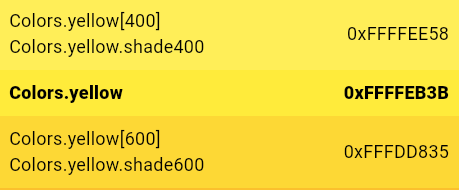
\includegraphics[width=0.33\textwidth]{imagenes/TerceraIteracion/ColorsYellow.png}
	\caption{Gama de colores amarillos de Flutter.}
\end{figure}

Para el fondo de la aplicación y algunos textos, se ha utilizado el blanco, Colors.white. 

\newpage

\subsubsection{Inicio y cierre de sesión}


En esta pantalla de inicio de sesión se utilizan campos de texto que permiten que el usuario proporcione las credenciales a la aplicación. Se hace uso de \textit{validator} para comprobar que los campos no se dejan vacíos. Si las credenciales son incorrectas al presionar \textit{Iniciar sesión}, aparece un diálogo similar al de cerrar sesión informando al usuario del problema. 

\begin{figure}[H]
	\centering
	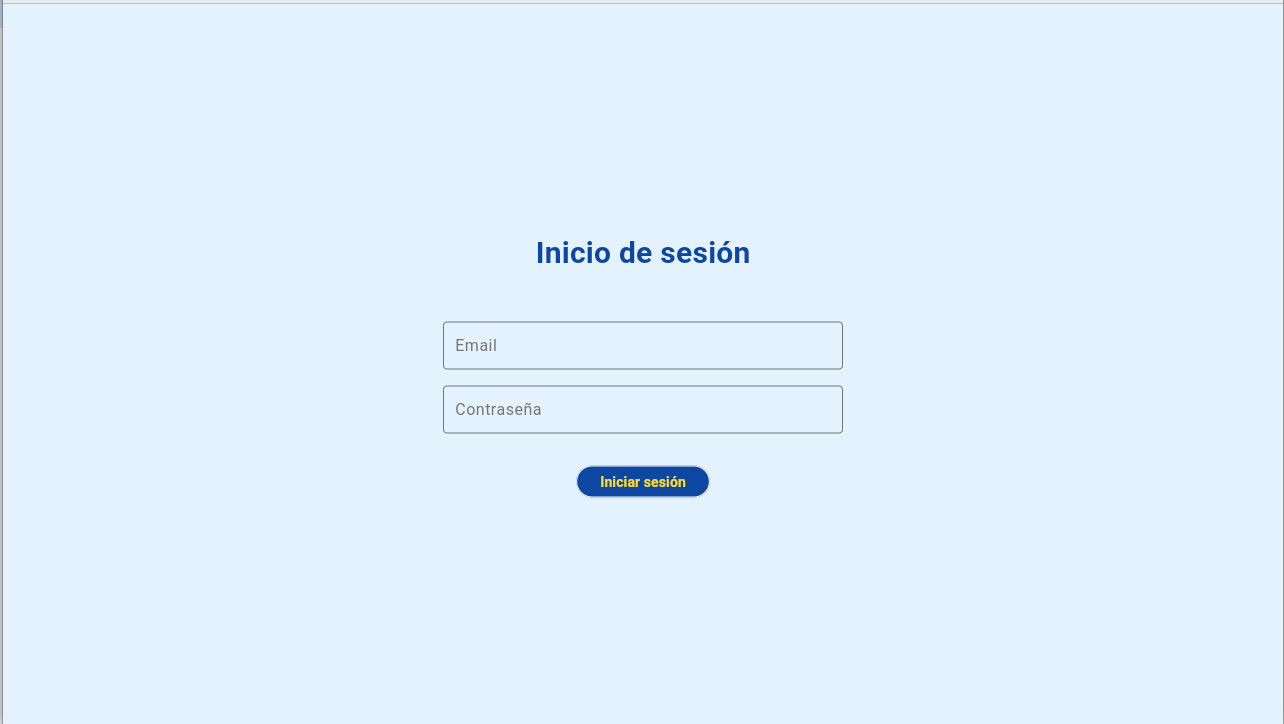
\includegraphics[width=0.7\textwidth]{imagenes/TerceraIteracion/login.png}
	\caption{Pantalla de inicio de sesión.}
\end{figure}

Al presionar el botón de \textit{Confirmar} del diálogo, se cierra la sesión activa del usuario. 

\begin{figure}[H]
	\centering
	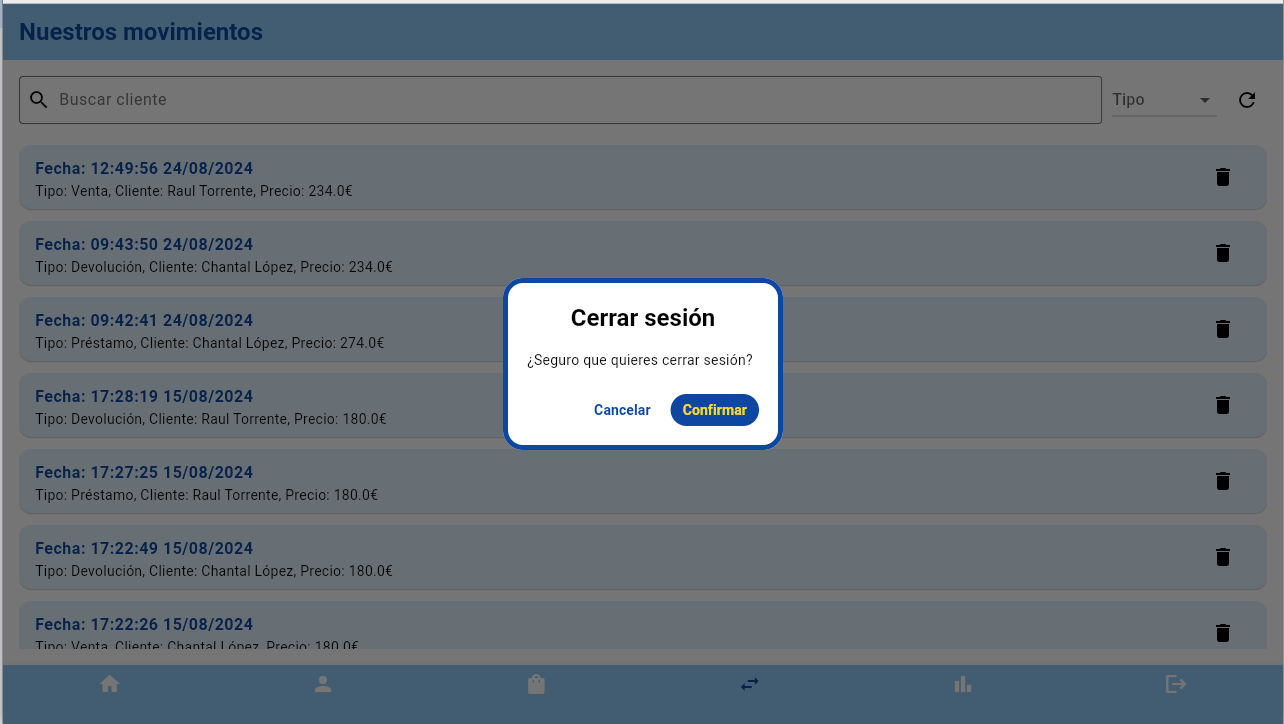
\includegraphics[width=0.7\textwidth]{imagenes/TerceraIteracion/logout.png}
	\caption{Cierre de sesión.}
\end{figure}

\newpage

\subsubsection{Pantalla principal}

Esta pantalla está compuesta por un campo de texto no editable, para mostrar las ganancias diarias, y dos \textit{ElevatedButton} que permiten crear una nueva venta o préstamo. 

\begin{figure}[H]
	\centering
	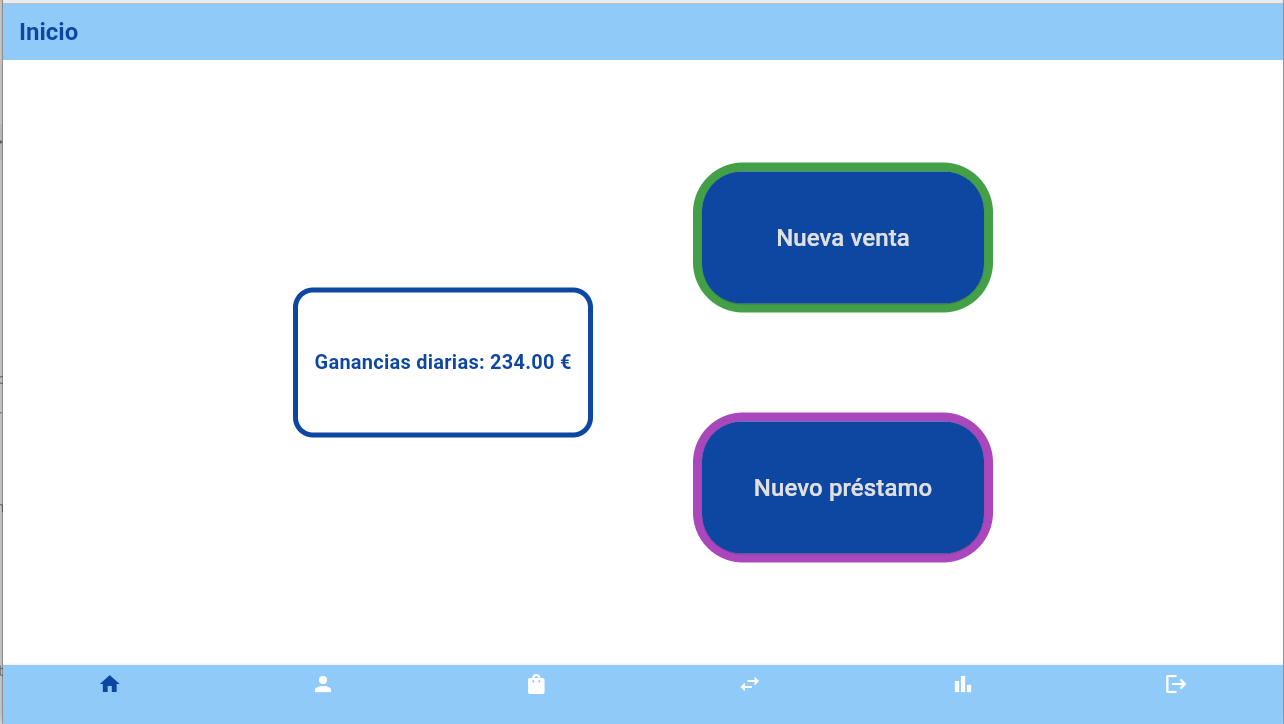
\includegraphics[width=0.7\textwidth]{imagenes/TerceraIteracion/mainPage.png}
	\caption{Pantalla principal.}
\end{figure}

La pantalla de \textit{Nueva venta} y \textit{Nuevo préstamo} parten de la misma implementación y se diferencian con un booleano que especifica el movimiento que se está creando. Para la búsqueda se utiliza un campo de texto que escucha cada cambio y encuentra los artículos dinámicamente. Una vez encontrado el artículo, los desplegables de \textit{Talla} y \textit{Color} realizan una consulta a la base de datos y ofrecen las opciones que tiene ese artículo para esos valores. La cantidad mínima es 1 y la cantidad máxima la determina la cantidad de stock que haya en la tienda. Si la cantidad seleccionada sobrepasa la cantidad existente en la tienda, se muestra un diálogo avisando de que la cantidad seleccionada es incorrecta y se muestra le cantidad posible. El precio, se va actualizando dinámicamente, multiplicando el precio del producto por la cantidad seleccionada de este. Al pulsar el símbolo \textit{+}, se genera una \textit{Card} con la información especificada y, a continuación, se puede añadir otro artículo a la factura. 

Si es una venta, el campo de cliente, puede dejarse vacío. Si es un préstamo, es obligatorio que se asigne un cliente ya que es un movimiento que no se paga en el momento. El campo de búsqueda del cliente funciona de la misma forma que la búsqueda del artículo. Si es una venta, aparece el desplegable para seleccionar el método de pago y es obligatorio rellenarlo, ya que deberá ser pagado en el momento. Ambos movimientos finalizan al presionar el botón de \textit{Aceptar}. 

Cada vez que se añade un nuevo movimiento, se manda una notificación mediante el uso de un \textit{Provider ChangeNotifier} para avisar de que el resto de pantallas deben actualizarse con la nueva información que se acaba de añadir. El resto de pantallas escuchan con un \textit{Consumer}. 

\begin{figure}[H]
	\centering
	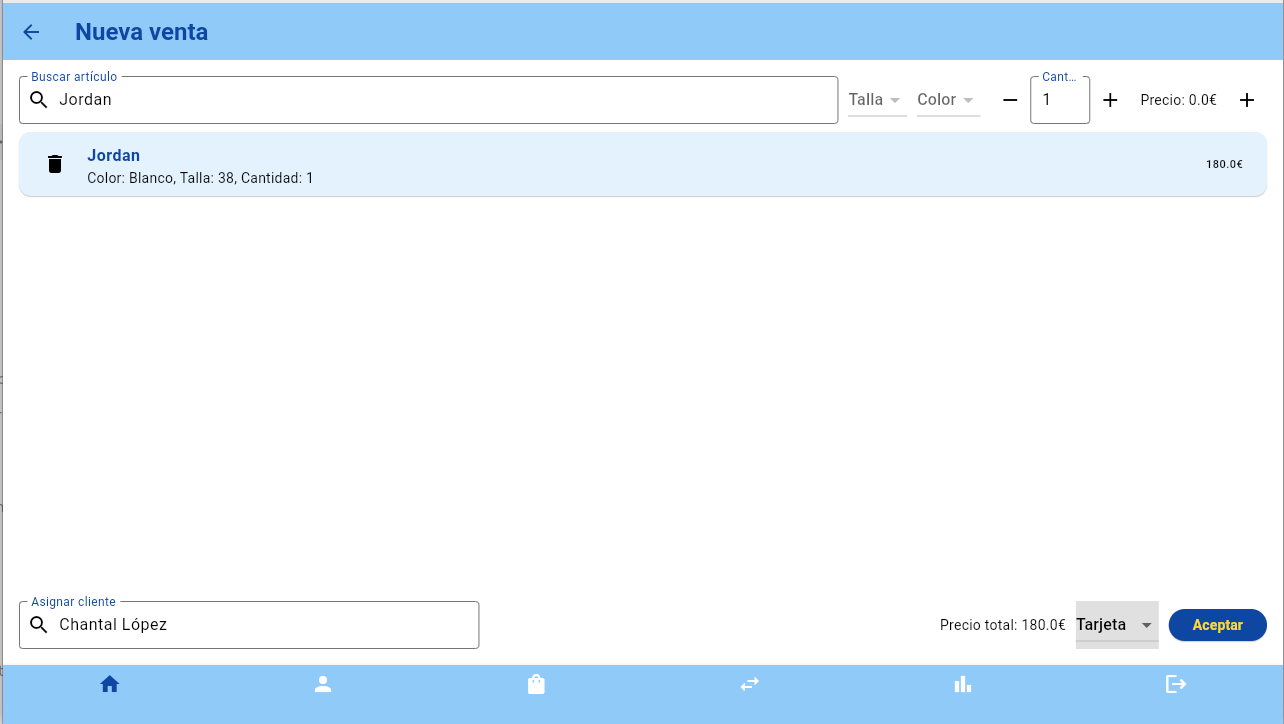
\includegraphics[width=0.7\textwidth]{imagenes/TerceraIteracion/nuevaVenta.png}
	\caption{Pantalla de nueva venta.}
\end{figure}

\begin{figure}[H]
	\centering
	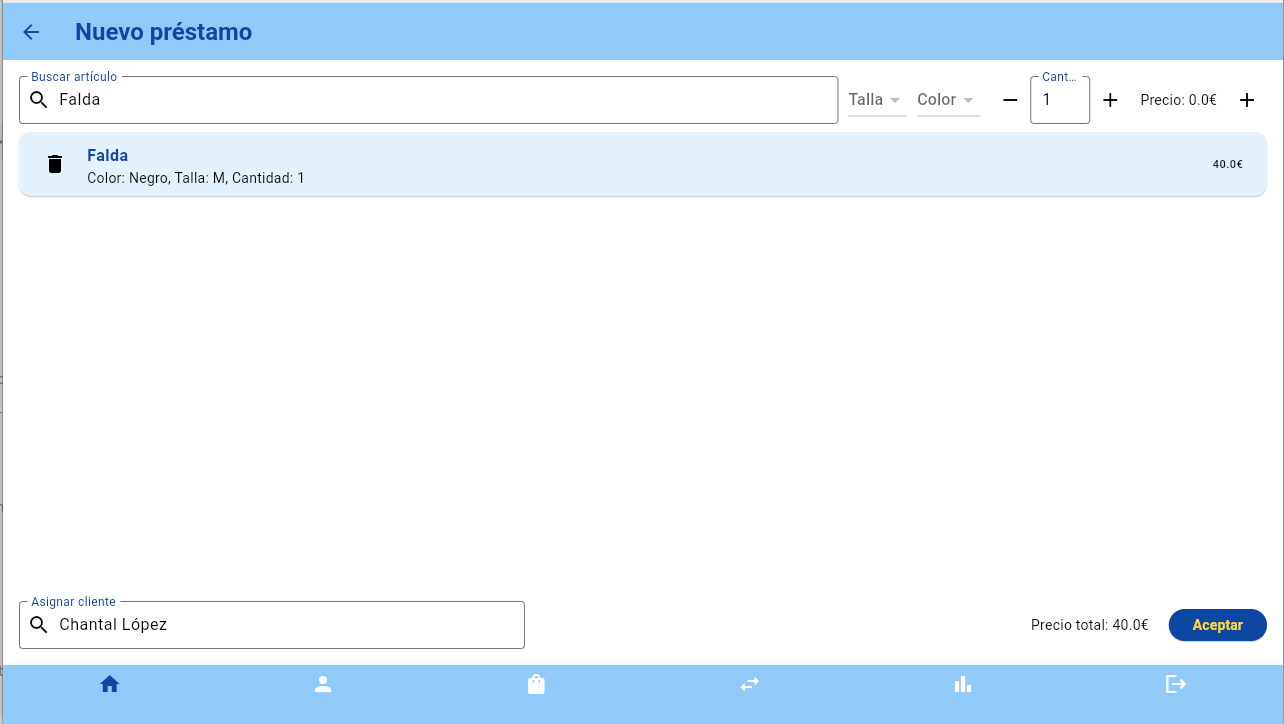
\includegraphics[width=0.7\textwidth]{imagenes/TerceraIteracion/nuevoPrestamo.png}
	\caption{Pantalla de nuevo préstamo.}
\end{figure}

\newpage

\subsubsection{Pantalla de clientes}

En esta pantalla, el buscador funciona de la misma forma que explicamos con anterioridad. A la derecha, podemos ver un icono de dinero que activa y desactiva un booleano para filtrar aquellos clientes que se encuentran en dinero negativo en la tienda. Además, en cada \textit{Card} de clientes con dinero positivo o negativo podemos ver una flecha. Esto se ha llevado a cabo como requisito que se añadió en la primera iteración. El cliente expresó que quería poder diferenciar el estado positivo o negativo del cliente no solamente con el color, sino también con algún símbolo, para aquellas personas que no diferencien los colores de forma correcta. Por tanto, se añadió una flecha hacia arriba o hacia abajo para ser más accesibles. 

La parte central de la pantalla es un \textit{StreamBuilder} que reconstruye su contenido cada vez que hay algún \textit{insert}, \textit{update} o \textit{delete}. De esta forma, el contenido que se muestra en la pantalla de visualización de los clientes, está siempre actualizado. Además, escucha los \textit{ChangeNotifier} con el \textit{Consumer} para actualizar los datos monetarios del cliente que se vean afectados con los movimientos de la tienda. 

Para eliminar un cliente, no debe de estar vinculado a ningún movimiento. Si está vinculado a un movimiento, debe de existir, para mantener el histórico de la tienda. 

\begin{figure}[H]
	\centering
	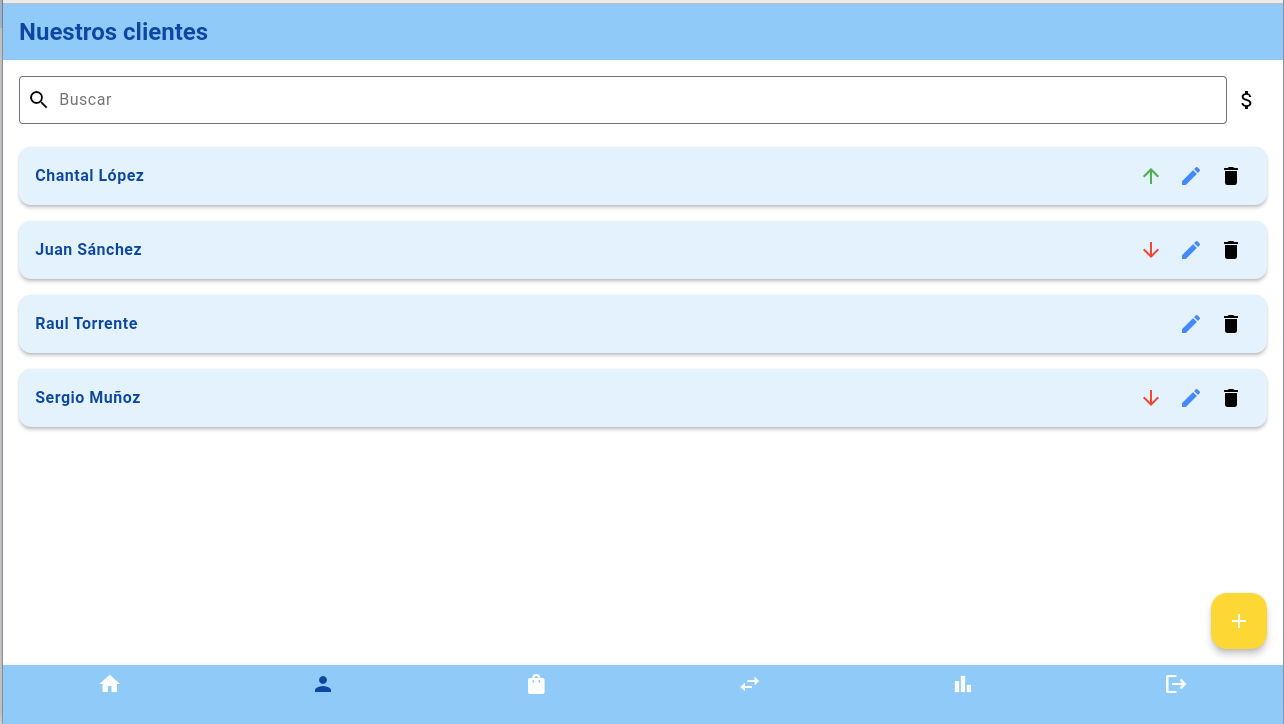
\includegraphics[width=0.7\textwidth]{imagenes/TerceraIteracion/clientView.png}
	\caption{Pantalla de visualización de clientes.}
\end{figure}

Las tres pantallas siguientes son muy similares. La primera de ellas, la que muestra los detalles, son unos campos de texto inicializados a los valores almacenados en la base de datos y con la propiedad \textit{readonly}. La segunda pantalla, la pantalla de edición, tiene los mismos campos de texto inicializados a dichos valores, pero sin la propiedad \textit{readonly} para permitir modificar la información. Además, se comprueba que el número de teléfono sea correcto mediante una expresión regular. En la tercera pantalla, la pantalla de registro, los campos no están inicializados y se comprueba que el nombre esté relleno mediante un \textit{validator}.  

\begin{figure}[H]
	\centering
	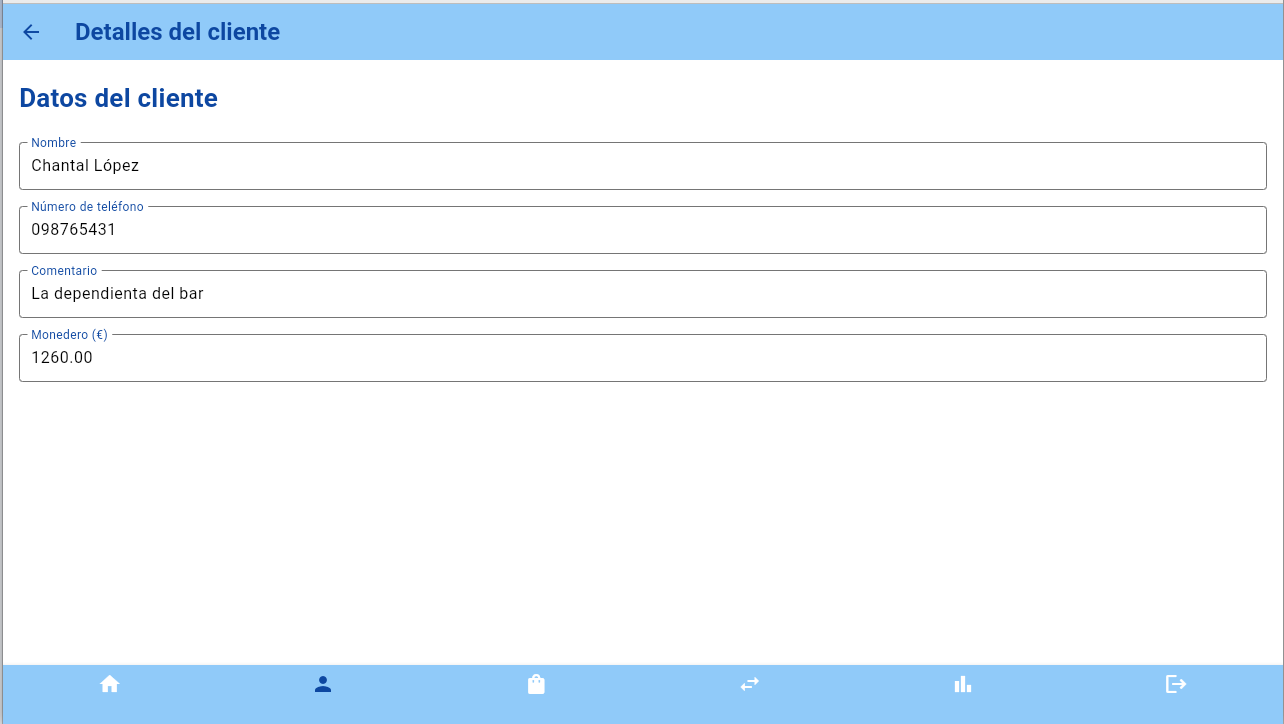
\includegraphics[width=0.7\textwidth]{imagenes/TerceraIteracion/clientDetails.png}
	\caption{Pantalla de visualización de los datos de un cliente.}
\end{figure}

\begin{figure}[H]
	\centering
	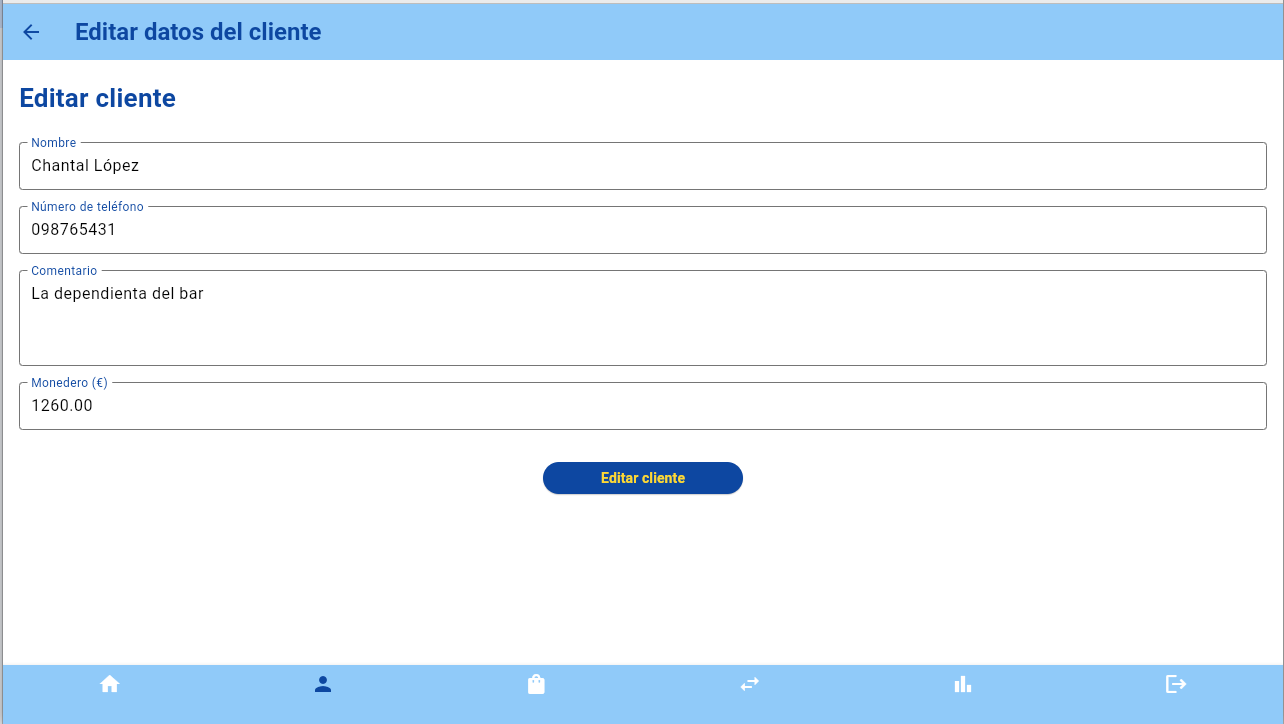
\includegraphics[width=0.7\textwidth]{imagenes/TerceraIteracion/clientEdit.png}
	\caption{Pantalla de edición de los datos de un cliente.}
\end{figure}

\begin{figure}[H]
	\centering
	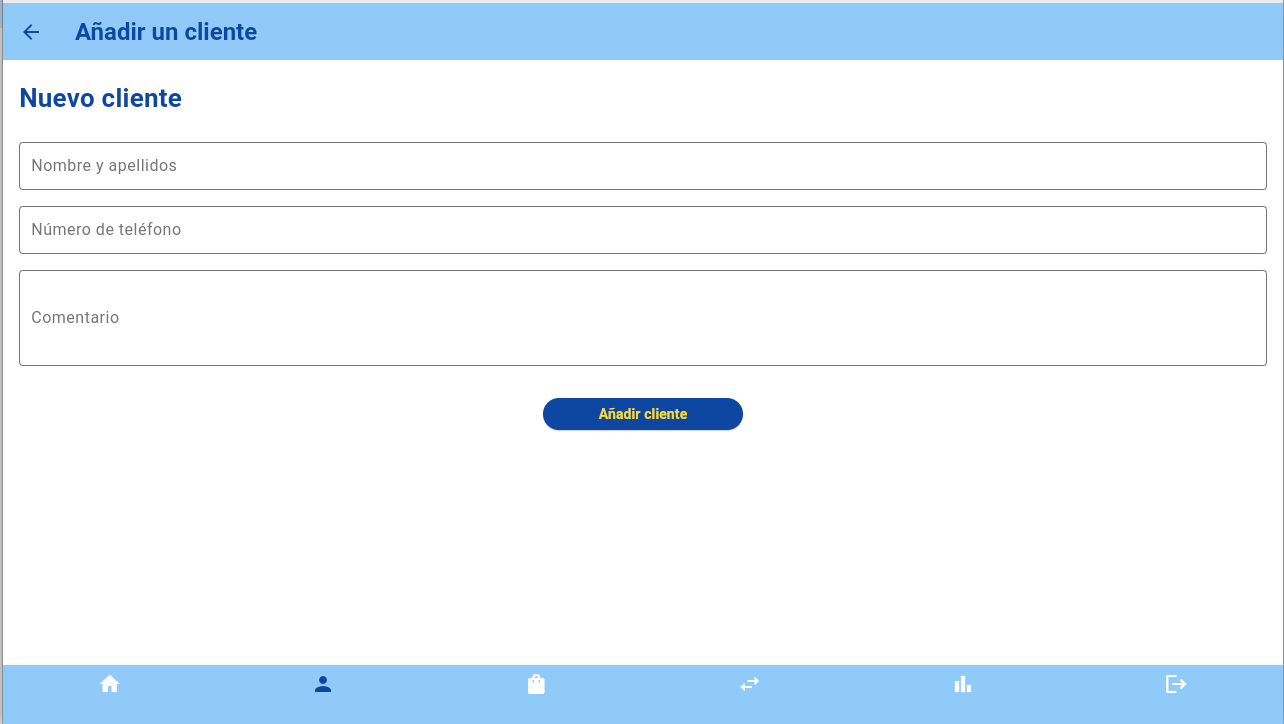
\includegraphics[width=0.7\textwidth]{imagenes/TerceraIteracion/newClient.png}
	\caption{Pantalla de registro de un nuevo cliente.}
\end{figure}

\newpage

\subsubsection{Pantalla de artículos}

Esta pantalla muestra las categorías en forma de \textit{Card} mediante un StreamBuilder, de la misma forma que se explicó en la pantalla de los clientes. Se puede añadir o editar una categoría, de la forma que se muestra en las siguientes imágenes. 

Para eliminar una categoría, no debe de tener artículos dentro de ella. 

\begin{figure}[H]
	\centering
	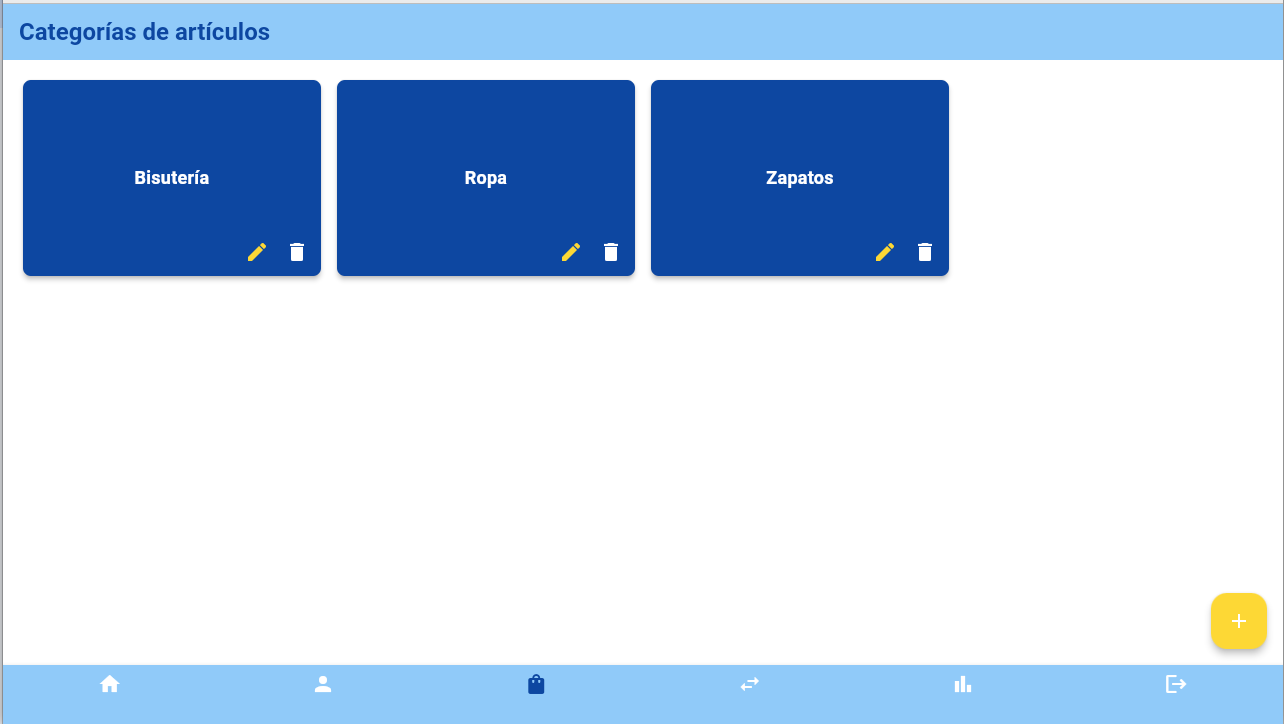
\includegraphics[width=0.7\textwidth]{imagenes/TerceraIteracion/categoryView.png}
	\caption{Pantalla de visualización de las categorías.}
\end{figure}

\begin{figure}[H]
	\centering
	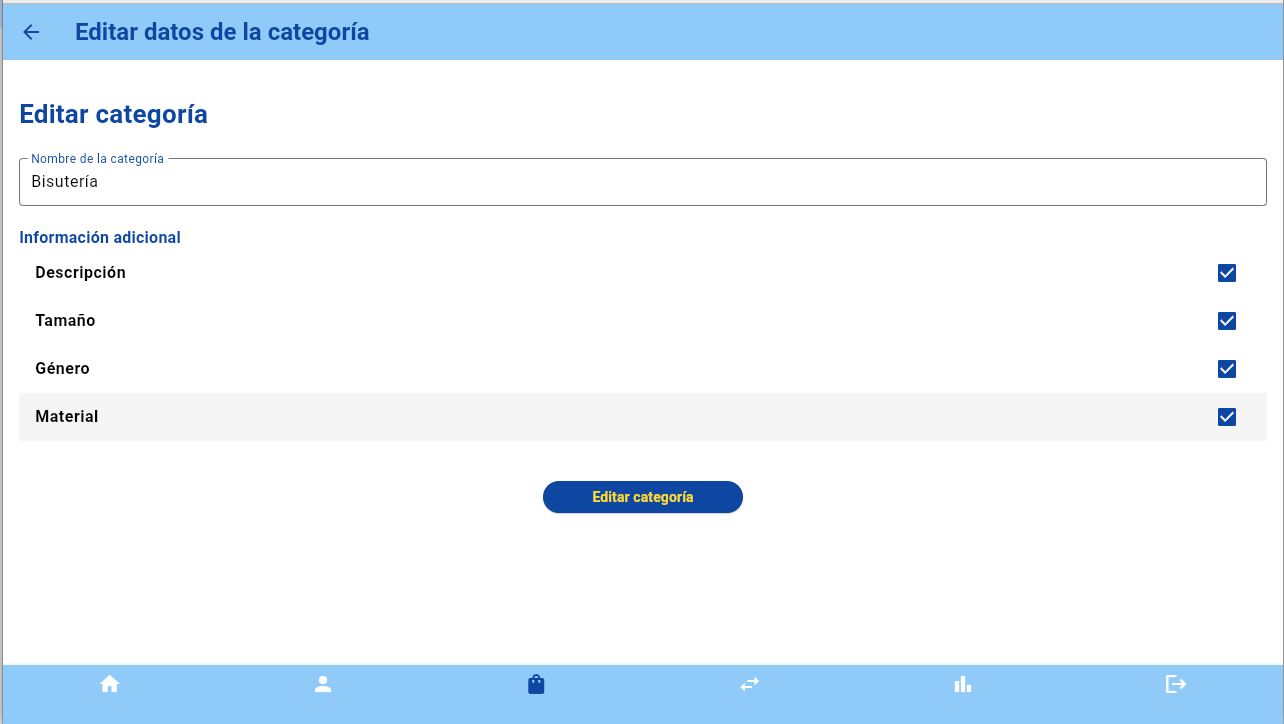
\includegraphics[width=0.7\textwidth]{imagenes/TerceraIteracion/categoryEdit.png}
	\caption{Pantalla de edición de las propiedades de una categoría.}
\end{figure}

\begin{figure}[H]
	\centering
	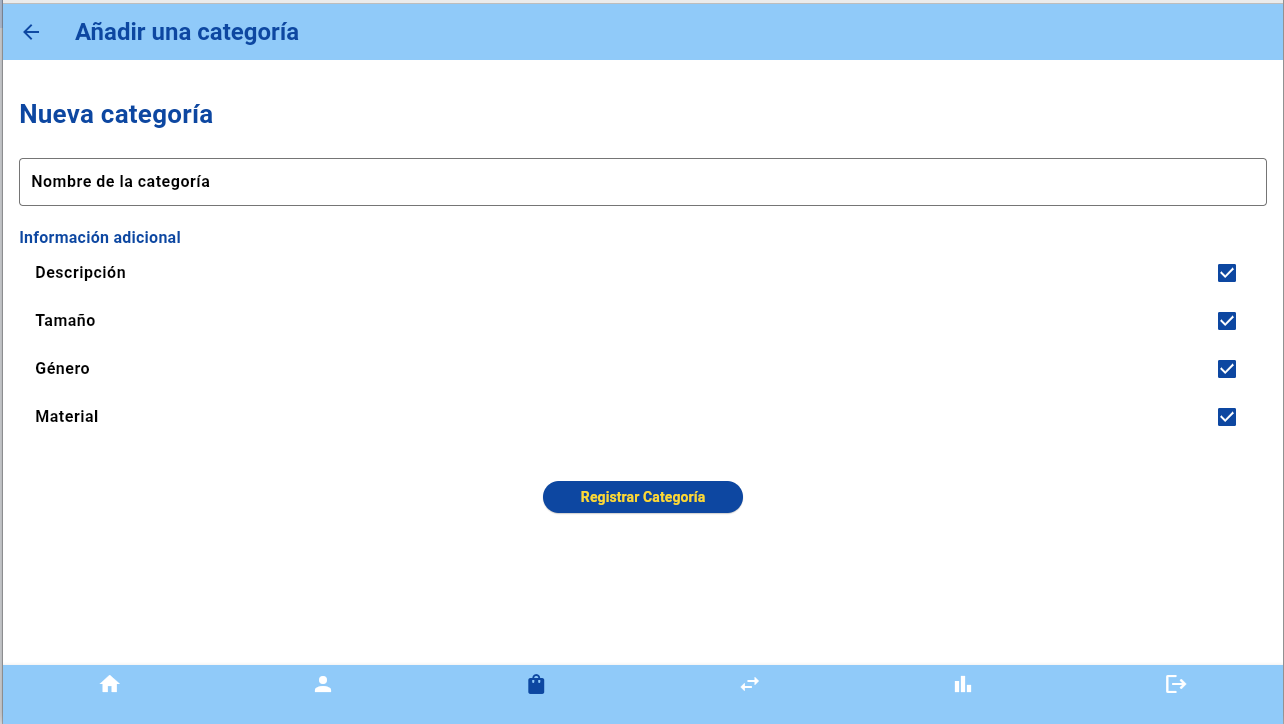
\includegraphics[width=0.7\textwidth]{imagenes/TerceraIteracion/newCategory.png}
	\caption{Pantalla de registro de una nueva categoría.}
\end{figure}

La pantalla de visualización de artículos es muy similar a la pantalla de visualización de clientes. Un aspecto a destacar es el desplegable de \textit{Subcategoría}. Este desplegable realiza una consulta en la base de datos y trae las posibles subcategorías de artículos dentro de esa categoría. Permite seleccionar una subcategoría y filtrar por dicha subcategoría. 

Para eliminar un artículo, no debe de estar vinculado a ningún movimiento. Si está vinculado a un movimiento, debe de mantenerse para mantener el histórico de la tienda. 

\begin{figure}[H]
	\centering
	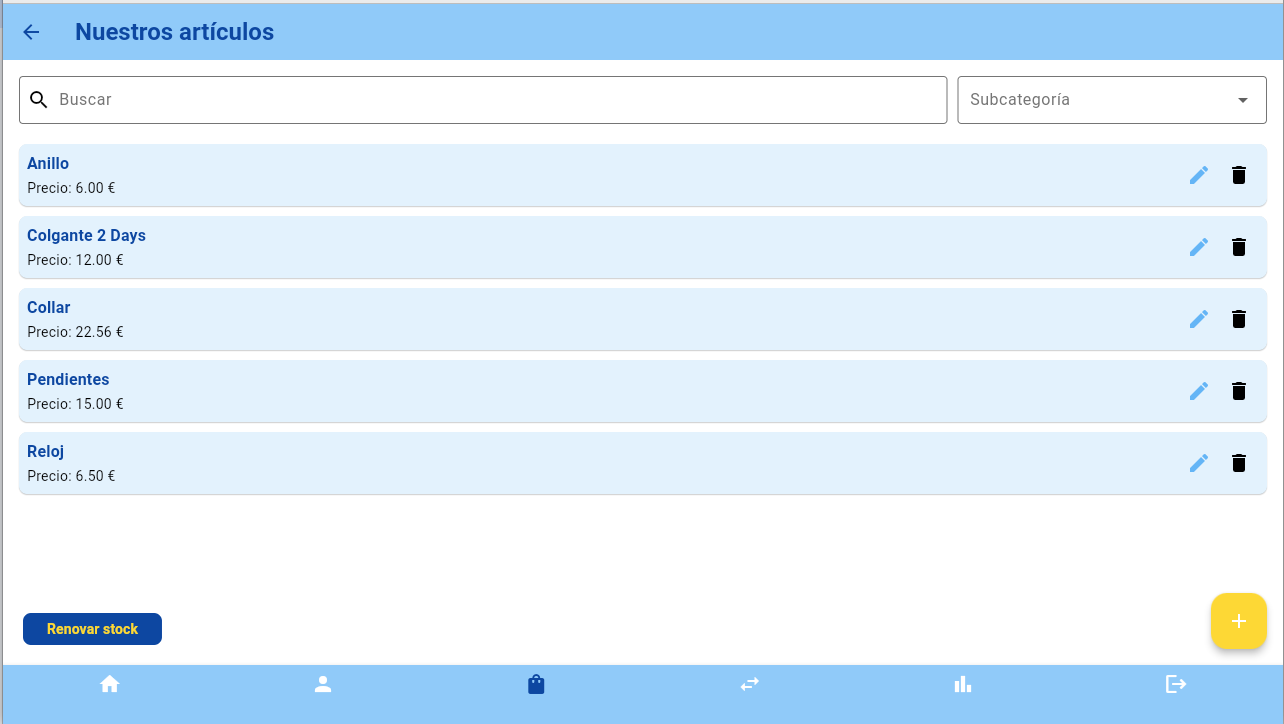
\includegraphics[width=0.7\textwidth]{imagenes/TerceraIteracion/articleView.png}
	\caption{Pantalla de visualización de los artículos de una categoría.}
\end{figure}

Las pantallas de visualización de los detalles de un artículo, editar o añadir son similares a las pantallas comentadas en el apartado de clientes. Al añadir un artículo, es obligatorio añadir mínimo una talla, se comprueba mediante un \textit{validator}. 

\begin{figure}[H]
	\centering
	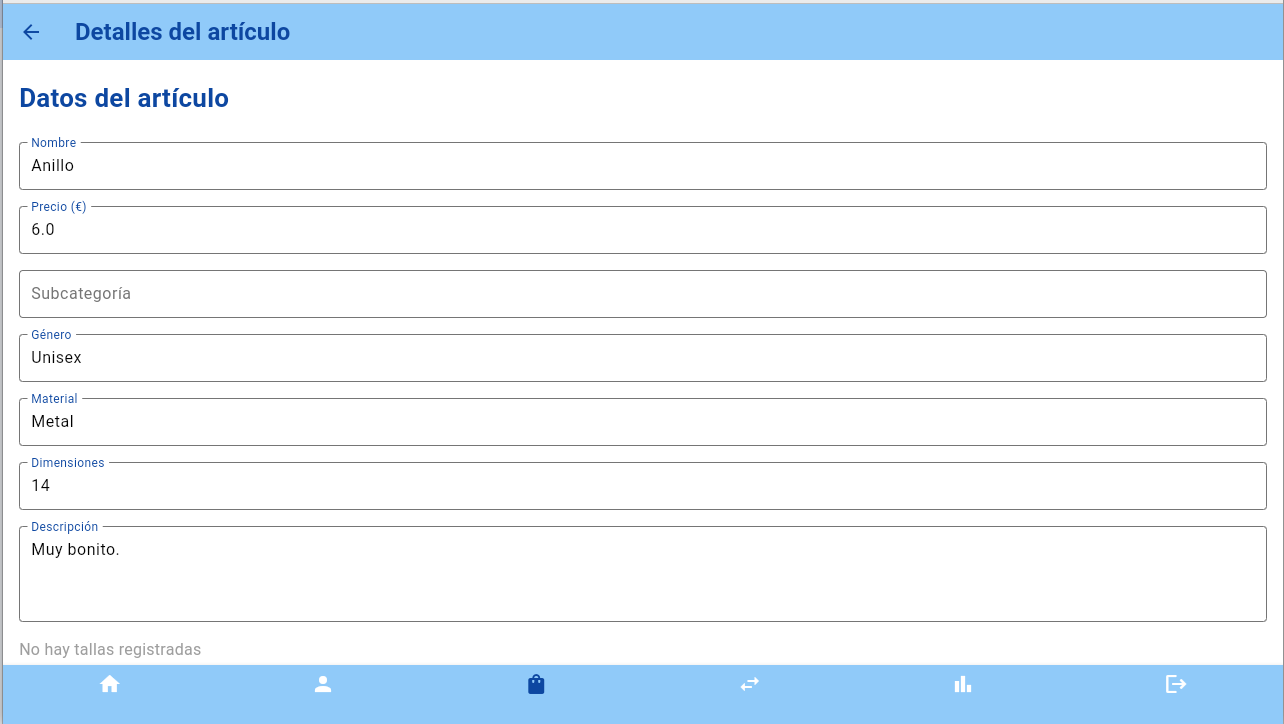
\includegraphics[width=0.7\textwidth]{imagenes/TerceraIteracion/articleDetails.png}
	\caption{Pantalla de visualización de los datos de un artículo.}
\end{figure}

\begin{figure}[H]
	\centering
	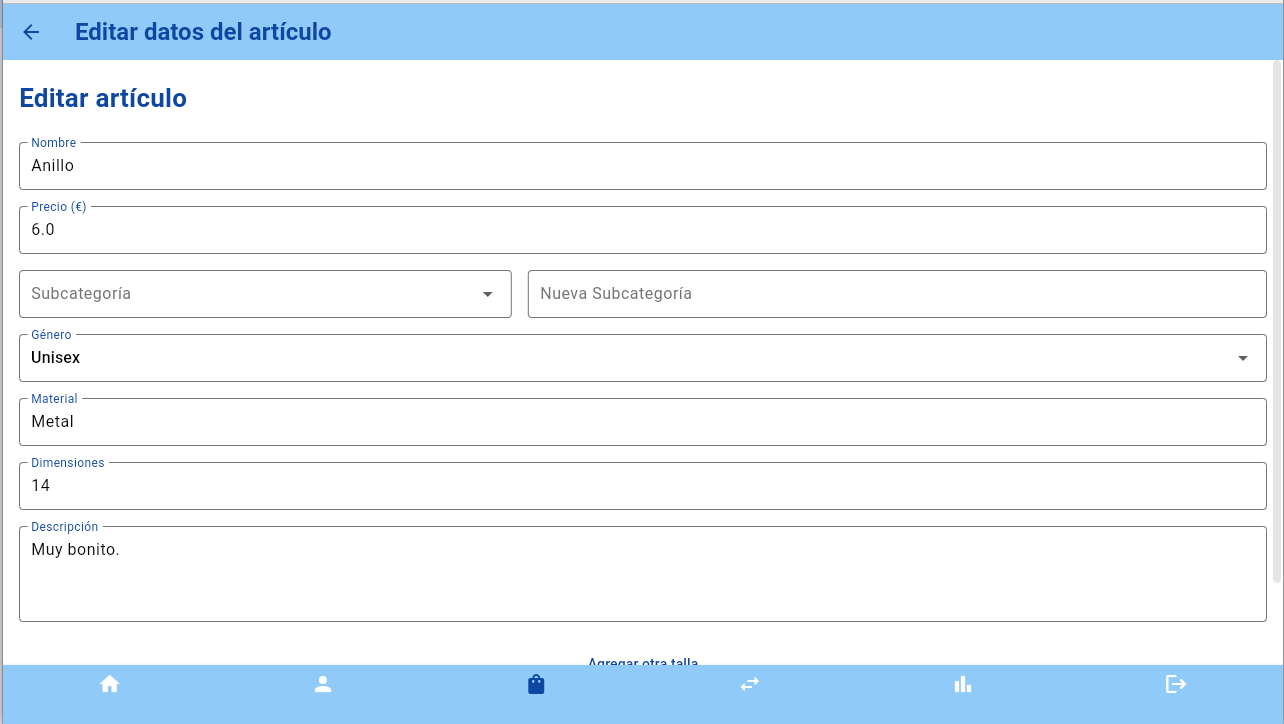
\includegraphics[width=0.7\textwidth]{imagenes/TerceraIteracion/articleEdit.png}
	\caption{Pantalla de edición de los datos de un artículo.}
\end{figure}

\begin{figure}[H]
	\centering
	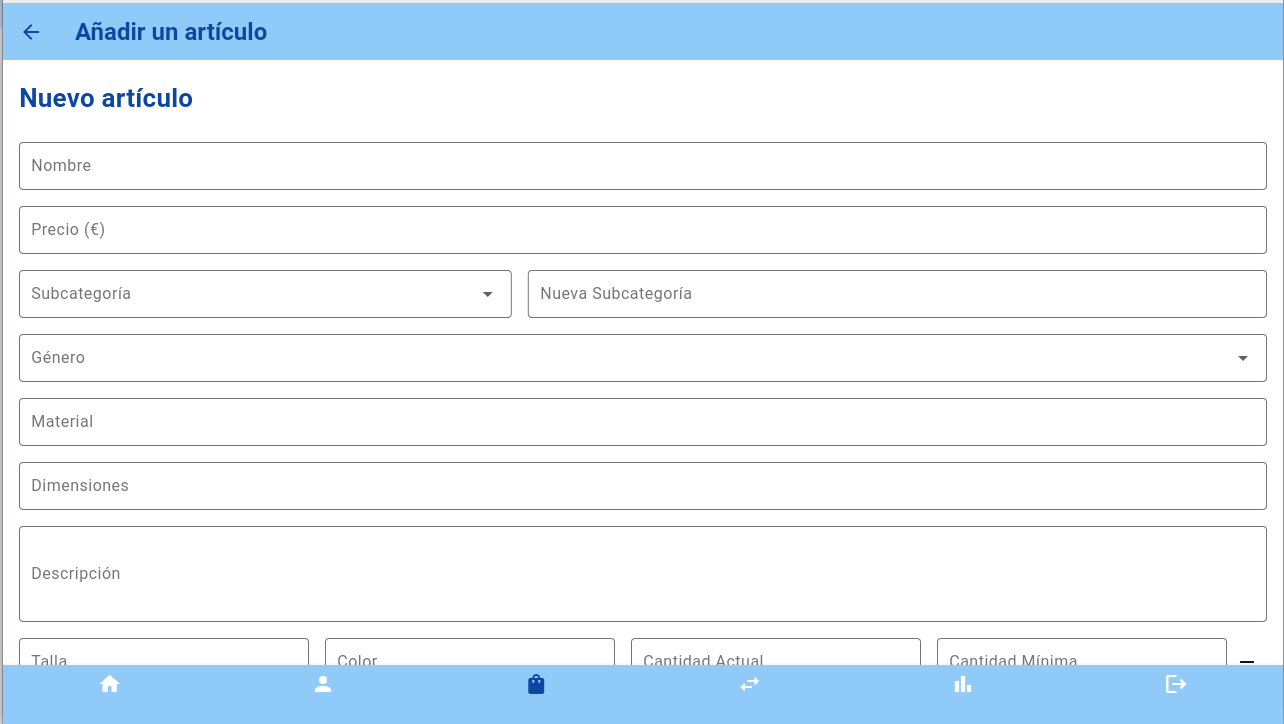
\includegraphics[width=0.7\textwidth]{imagenes/TerceraIteracion/newArticle.png}
	\caption{Pantalla de registro de un nuevo artículo.}
\end{figure}

\newpage

La pantalla de stock muestra los artículos cuya cantidad actual es crítica y necesita ser renovada. Se muestra mediante campo de texto \textit{readonly}.

\begin{figure}[H]
	\centering
	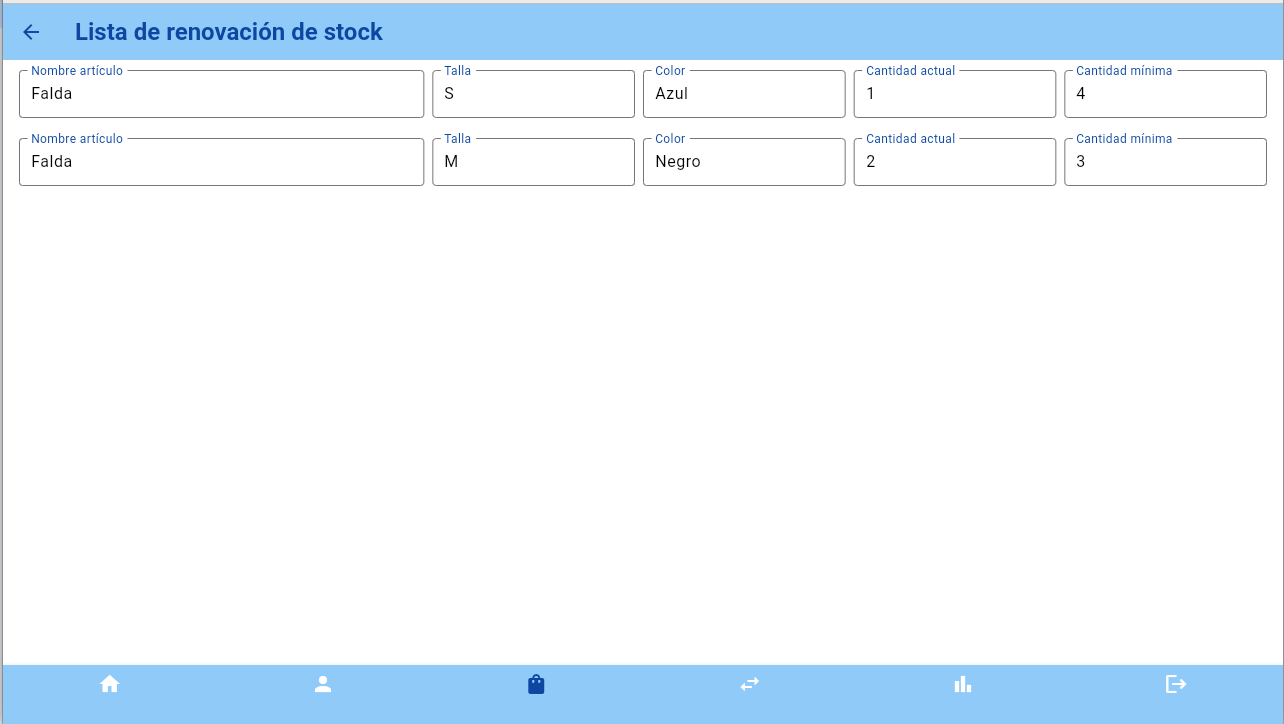
\includegraphics[width=0.7\textwidth]{imagenes/TerceraIteracion/stock.png}
	\caption{Pantalla de visualización la lista de renovación del stock.}
\end{figure}

\newpage

\subsubsection{Pantalla de movimientos}

La pantalla de visualización de movimientos es similar a las anteriores que muestran todas las instancias almacenadas. La búsqueda permite buscar movimientos de un cliente en específico. El desplegable filtra por tipo de movimiento, por lo que permite seleccionar \textit{Venta}, \textit{Préstamo} o \textit{Devolución}. La rueda situada en la derecha sirve para quitar la selección del desplegable. 

Para la parte central, donde se muestran los movimientos en forma de \textit{Card}, se utiliza un \textit{StreamBuilder} que reconstruye su contenido cada vez que hay algún \textit{insert}, \textit{update} o \textit{delete}. De esta forma, el contenido que se muestra en la pantalla de movimientos, está siempre actualizado. El icono de la papelera permite eliminar un movimiento solo si no está vinculado a otro. Si no se puede eliminar, se muestra un diálogo avisando del motivo.   

\begin{figure}[H]
	\centering
	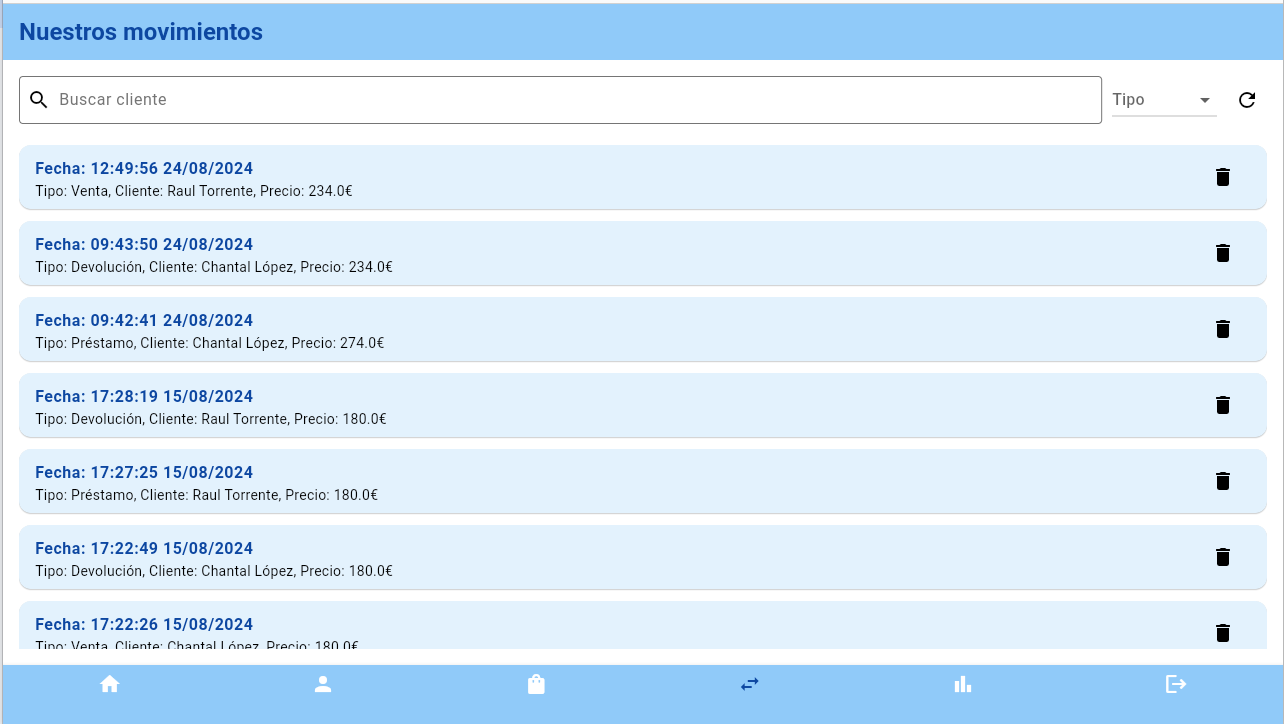
\includegraphics[width=0.7\textwidth]{imagenes/TerceraIteracion/movementsView.png}
	\caption{Pantalla de visualización los movimientos de la tienda.}
\end{figure}

Esta pantalla recoge muchas funcionalidades y muestra unas u otras en función del tipo de movimiento y su estado. Para \textit{Ventas}, si no se ha hecho una devolución anteriormente, se muestran dos botones en la parte superior que permiten realizar una devolución parcial o total. Si se decide una devolución total de la venta, se muestra un diálogo de confirmación. Al confirmar, se crea un movimiento de devolución con los datos de la venta. Si se elige una devolución parcial, la interfaz de la visualización de los detalles del movimiento cambia ligeramente y se asemeja a la creación de una \textit{Nueva venta}. Permite seleccionar los artículos que se desean devolver y el método de pago con el que se desea recibir la devolución. Esto se consigue con un \textit{booleano} que cambia de estado al pulsar el botón de \textit{Devolución parcial}. Si está activo, desaparecen algunos campos de detalle del movimiento para mostrar los elementos que permiten la creación de la devolución parcial. Cuando una venta sí que tiene una devolución hecha, ambos movimientos se vinculan. En la parte superior derecha desaparecen los dos botones que se comentaban antes y aparece un botón que te lleva directamente a los detalles de la devolución. En la devolución también estará ese mismo botón que te redirige a la venta de la que proviene dicha devolución. De esta forma, ambos movimientos están relacionados entre ellos. 

Si es un \textit{Pŕestamo}, funciona de la misma forma que la venta, pero en lugar del botón de \textit{Devolución parcial}, estará el botón de \textit{Compra}. Este botón te redirige a la misma pantalla de selección de artículos y creación de movimientos de la que hablábamos anteriormente. Sin embargo, se llama a otro método distinto, ya que los artículos seleccionados serán comprados en vez de devueltos. Además, los artículos que no se seleccionen, se mostrarán reflejados en un movimiento de devolución. Por tanto, al pulsar este botón, se podrán comprar todos los artículos, generando un único movimiento de \textit{Venta} o se podrá hacer una compra parcial, generando dos movimientos: una \textit{Venta} con los artículos seleccionados y una \textit{Devolución} con los artículos que restan. 

Si es una \textit{Devolución}, únicamente se podrán ver los detalles de la devolución y se podrá utilizar el botón de la parte superior derecha para ir al movimiento del que proviene. 

\begin{figure}[H]
	\centering
	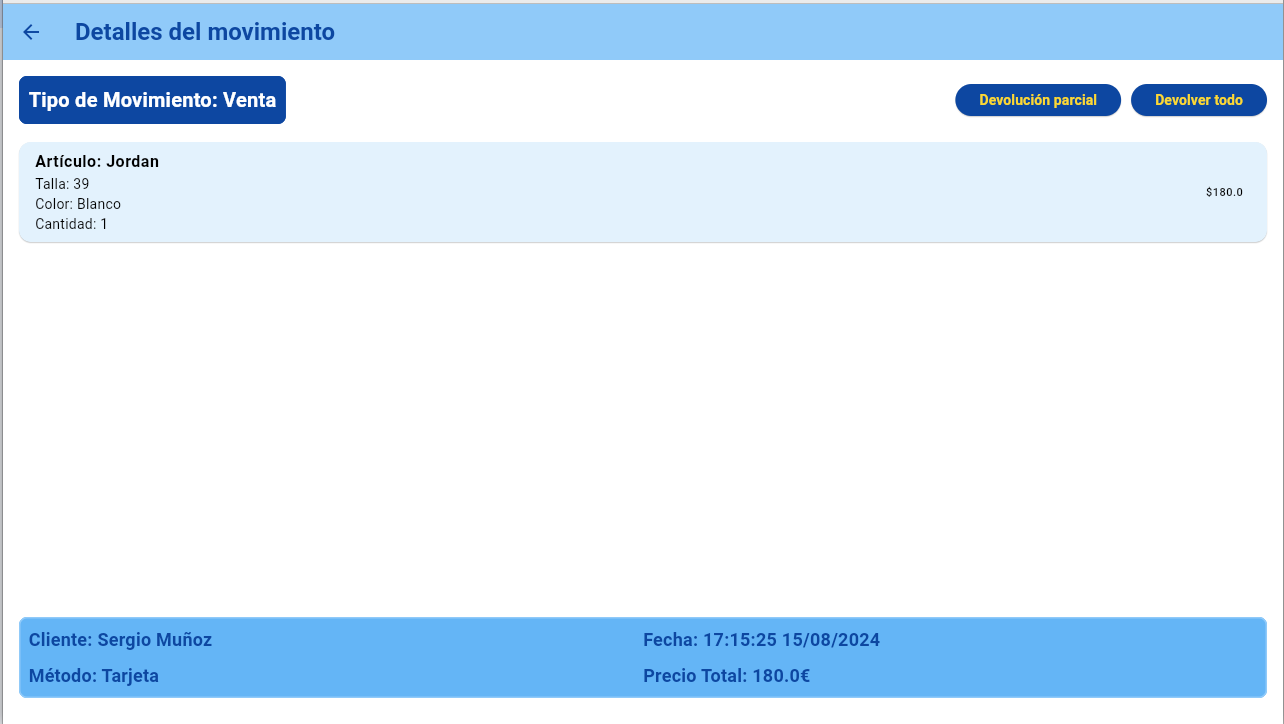
\includegraphics[width=0.7\textwidth]{imagenes/TerceraIteracion/movementDetails.png}
	\caption{Pantalla de visualización de los detalles de un movimiento.}
\end{figure}

\newpage

\subsubsection{Pantalla de gráficos}

Esta pantalla muestra un resumen de las ganancias de forma mensual o anual, según se elija en el desplegable de la parte superior derecha. Para conseguir ser más accesibles, las estadísticas positivas no solo se muestran con el color verde, sino que también se reflejan positivas en el eje. Las estadísticas negativas, se reflejan en la parte inferior del eje, además del color rojo. Esto se realiza con el pensamiento de las personas daltónicas que no puedan diferenciar los colores. De esta forma, quedan claras cuáles son las ganancias y cuáles son las pérdidas prestando atención al eje de la izquierda. 

\begin{figure}[H]
	\centering
	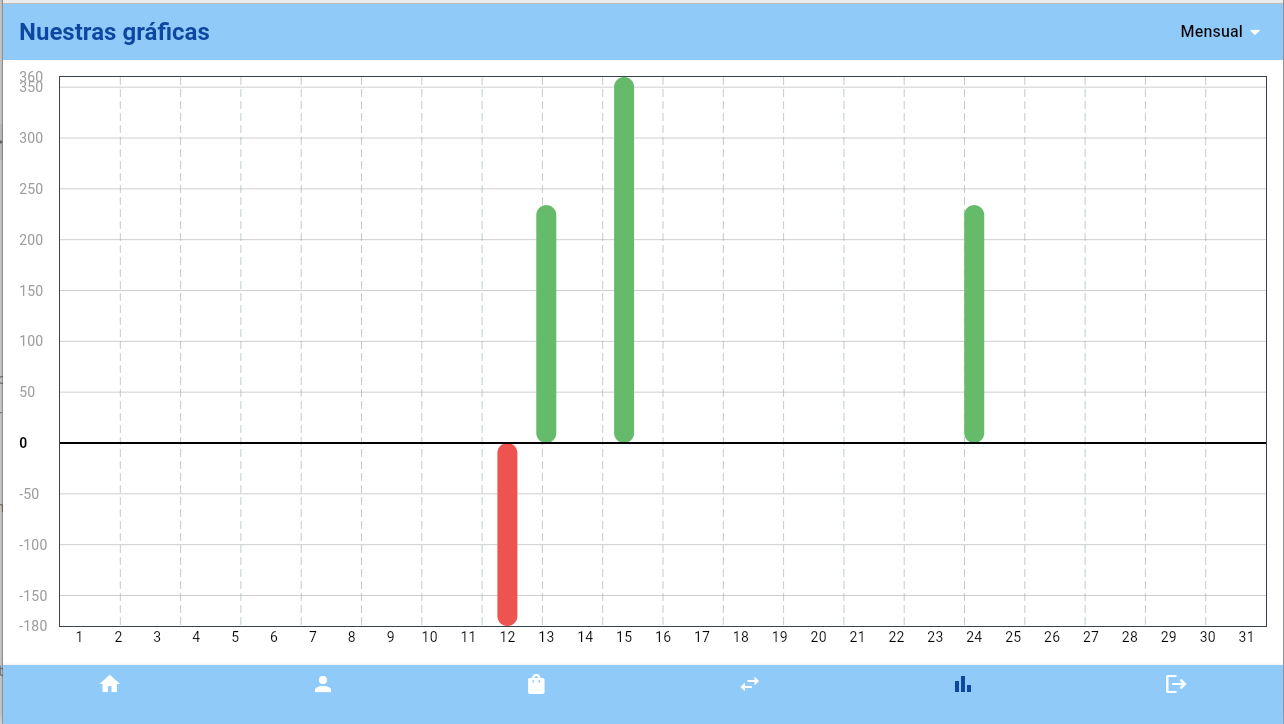
\includegraphics[width=0.7\textwidth]{imagenes/TerceraIteracion/graficosMensual.png}
	\caption{Pantalla de gráficos en modo mensual.}
\end{figure}

\subsection{Pruebas de funcionalidad}

Para testear la implementación que se ha llevado a cabo, se han realizado una serie de pruebas de funcionalidad: 

\begin{itemize}
	\item Comprobación de la representación de las ganancias del negocio en modo mensual. 
	\item Comprobación de la representación de las ganancias del negocio en modo anual. 
\end{itemize}

\subsection{Revisión de la iteración}

Tras terminar la iteración, se le mostró al usuario el resultado y estuvo contento con el cambio de interfaz y la representación de las gráficas. Le resultó sencillo navegar por la aplicación gracias al etiquetado superior y le resultó intuitiva para operar. Además, también agradeció que se hubiera mejorado la accesibilidad de la aplicación. 

